%\chapter{<<Яичница, телек, герани цветы!>>}
%\chapter{Мярандукса}
%\chapter{Иггдрасиль}
\chapter{Компотик}
%\corner{64}
\vepsianrose

Адмирал проснулся, нащупал часы. Выспался он замечательно, ночь была тёплой и безветреной. На часах было около половины девятого, Замполит ещё спал. Адмирал повернулся на другой бок и подумал, что с погодой им, пока что, относительно везёт\mdash ночь выдалась такой тёплой, что пришлось даже скинуть тельняшку.

\diagdash Что, пора?\mdash сонно протянул Замполит.

\diagdash С добрым утром! Пора!\mdash Адмирал c трудом оделся и~собирался вылезать из палатки.

\diagdash С добрым, я поваляюсь чутка ещё.

\diagdash Я пошёл завтрак готовить!\mdash он выполз из~палатки и~увидал Пашу, который уже с удочкой наготове шёл к~берегу.

\diagdash Сань, чё на завтрак?\mdash Пашка насаживал наживку.

\diagdash Всё по классике, каша чемпионов!\mdash Адмирал хлопал себя по карманам штормовки в поисках закурить.

Вскоре проснулись и Серёга с Русланом. Адмирал быстренько развёл костёр, сделал утренний чай, поставил кашу вариться, а сам принялся измельчать ножом орехи и~сухофрукты для добавления в~кашу\mdash тот самый завтрак чемпионов\mdash высококалорийная еда, на которой они и~держались, фактически, весь день до ужина, делая только один\sdash два перекуса батончиками спортпита вместо обеда. Словом, кураги, чернослива и орехов он сыпал в~овсянку не~жадничая, от души.

День разгорался тёплый, солнечный. И если с~самого утра на небе не было ни облачка, то сейчас, когда приготовление завтрака было почти окончено, над озером повисли красивые кучерявые белые облачка. Настроение у~всех было отличнейшим\mdash народ традиционно собрался в кружок у костра. Адмирал и Замполит доделывали бутерброды с плавленым сыром и~копчёной колбасой, на~земле у костровища стояли миски в ожидании раздачи каши. Когда всё было готово, Адмирал взял крышку котелка и~постучал по ней половником:

\diagdash Ку\sdash у\sdash ушать! Айда на раздачу!\mdash он быстренько раскидал большим половником кашу по тарелкам и закрыл котелок.\mdash Бутеры с колбаской не~забываем! Кушаем хорошо, сегодня у нас интересный насыщенный день! И~погодка\sdash то гляньте какая! Шик!

\diagdash Шу-у-урик, отсюда поподробнее, п\sdash жалста! Каков план?\mdash попросил Серёга, остужая кашу в тарелке, из~которой шёл~пар.

\diagdash Да, что у нас сегодня?\mdash Руслану, как и остальным, были интересны планы на день.

Все расселись в кружок на походных стульчиках и креслах, трепезничали. Адмирал наворачивал овсянку с~сухофруктами:

\diagdash Ща, дайте заправиться\sdash то!\mdash и, утолив лёгкий утренний голод и переведя дух, продолжил:\mdash Сегодня у нас вторая часть <<Венеции>>\mdash будет ещё один канал, а потом по~цепочке озёр лопатим дальше, рек не будет.

\diagdash То есть течения не будет весь день, упахиваемся вёслами\mdash это я вам перевожу c адмиральского!\mdash ввернул, хохотнув, Паша.

\diagdash Не, упахиваться не будем, сегодня по плану пройдём меньше, чем вчера\mdash надо дать рукам втянуться в~греблю. Если вчера мы все были на энтузиазме и~подъёме, то~сегодня ходовой день может показаться сложнее вчерашнего. Поэтому сегодня не более 10\thinspace\nobreakdash---\thinspace 12 километров. По стоячей озёрной воде этого будет вполне достаточно.\mdash закончил Адмирал и откинулся на спинку кресла, потягивая чаёк с~бутером.

\diagdash А что насчёт каналов?\mdash уточнил Замполит.

\diagdash Ну, сегодня один канал точно, а дальше как пойдёт$\ldots$\mdash Адмирал прихлебнул крепкий утренний чай.

\diagdash Шурик$\ldots$ Это твоё коронное <<как пойдёт>>$\ldots$

\diagdash Так! Тащ Замполит! Спецом для тебя поясняю\mdash это означает, что если пройти по каналам не удастся, то пойдём по короткой речушке, соединяющей Торосозеро с~озером Мярандукса.

\diagdash Во\sdash о\sdash от! Это уже чуть больше конкретики,\mdash Киря прикурил от костра и откинулся в кресле,\mdash а то вечно у тя какие\sdash то сюрпризы.

\diagdash Никаких сюрпризов, аллес унтер контролле! Так, ещё чаю поставьте\mdash надо залить в термосы, и потихоньку начинаем паковаться.\mdash распорядился Адмирал.

Стоянку они покинули только в половину первого, сборы проходили совершенно лениво и не слишком организованно. Адмирал всегда учитывал эту особенность второго дня похода\mdash людям надо пройти слаживание, привыкнуть что и куда паковать, как размещать снарягу в~байдарке. Ну и, в целом, должен установиться ритм похода, на это тоже нужно время, примерно 2\thinspace\nobreakdash---\thinspace 3 дня. К~третьему дню команда, как правило, уже представляет собой более или менее слаженный организм. 

%\renewcommand*{\thefootnote}{\arabic{footnote}}
\renewcommand*{\thefootnote}{\fnsymbol{footnote}}
\setcounter{footnote}{0}
Адмиральская байдарка была готова первой\mdash Руслан и~Паша собрались и перетаскали вещи, потом помогли Шурику всё распихать под борта. Серёга с Кирей всё ещё возились с~упаковкой, а когда настал их черёд погрузки герм в байдарку, Шурику пришлось отчалить и~отойти от~берега\mdash места не хватало под зачаливание двух байдарок. Адмиральский экипаж отошёл от~берега и~лёг~в~дрейф\footnote{Дрейф (от гол. drijven\mdash плавать, гнать)\mdash снос движущегося судна с линии его курса под влиянием ветра, течений и др. причин. <$\ldots$> судно, не имеющее хода, лежит в дрейфе\cite{МорскойСправочник}.}. Внезапно ветер стал усиливаться, Адмирал оживился. Пашка обернулся на носу байды:

\diagdash Ты думаешь о том же, о чём и я?

\diagdash Ставь парус!!!\mdash отдал Адмирал команду, ему очень хотелось попробовать как пойдет байдарка под даже таким простым и небольшим парусом. Прямо перед походом он приобрёл складной парус, который представлял собой полусферу с прозрачной вставкой\mdash чтобы видеть, куда плывёшь\mdash и с тонким стальным тросом, вшитым по кругу для придания формы. Всю эту конструкцию можно было сложить в круг небольшого диаметра, так что сложенный парус легко помещался в грузовом отсеке байды.


\begingroup
\justifying
\parfillskip=0pt % <- это заставит последнюю строку растягиваться

\renewcommand*{\thefootnote}{\arabic{footnote}}
\setcounter{footnote}{0}
Пашка разобрался с такелажем\footnote{Совокупность судовых снастей, в т.ч. для управления парусами\cite{МорскойСправочник}.}, привязал шкоты\footnote{Снасть бегучего такелажа, с помощью которой <...> оттягивают назад углы парусов\cite{МорскойСправочник}.} к~стальному тросу, приладил нижнюю часть паруса на~носовом шпангоуте и, наконец, полностью подготовившись, передал Адмиралу назад своё весло и взял в~руки шкоты, ловя ветер:

\par
\endgroup

\noindent
\begin{minipage}{0.38\textwidth}
	\setlength{\parindent}{1.0cm}  % Включаем красную строку
	\setlength{\parskip}{0.25cm}     % Межабзацный отступ, как в основном тексте
	
	\vspace{-0.4cm}
	\diagdash И\sdash и\sdash иха! 
	
	\diagdash ПОТАЩИЛО!!! --- Адмирал в полном восторге перестал грести веслом по\sdash байдарочному и~взял его под мышку на манер руля.\mdash Погнали!!!
	
	Ветер дул, конечно, не~особо сильный, но этого было вполне достаточно, чтобы дать им ход в~парочку км/ч. Второй экипаж, тем временем, наконец\sdash то отчалил и~догнал их:
\end{minipage}\hfill
\begin{minipage}{0.57\textwidth}
	\centering
	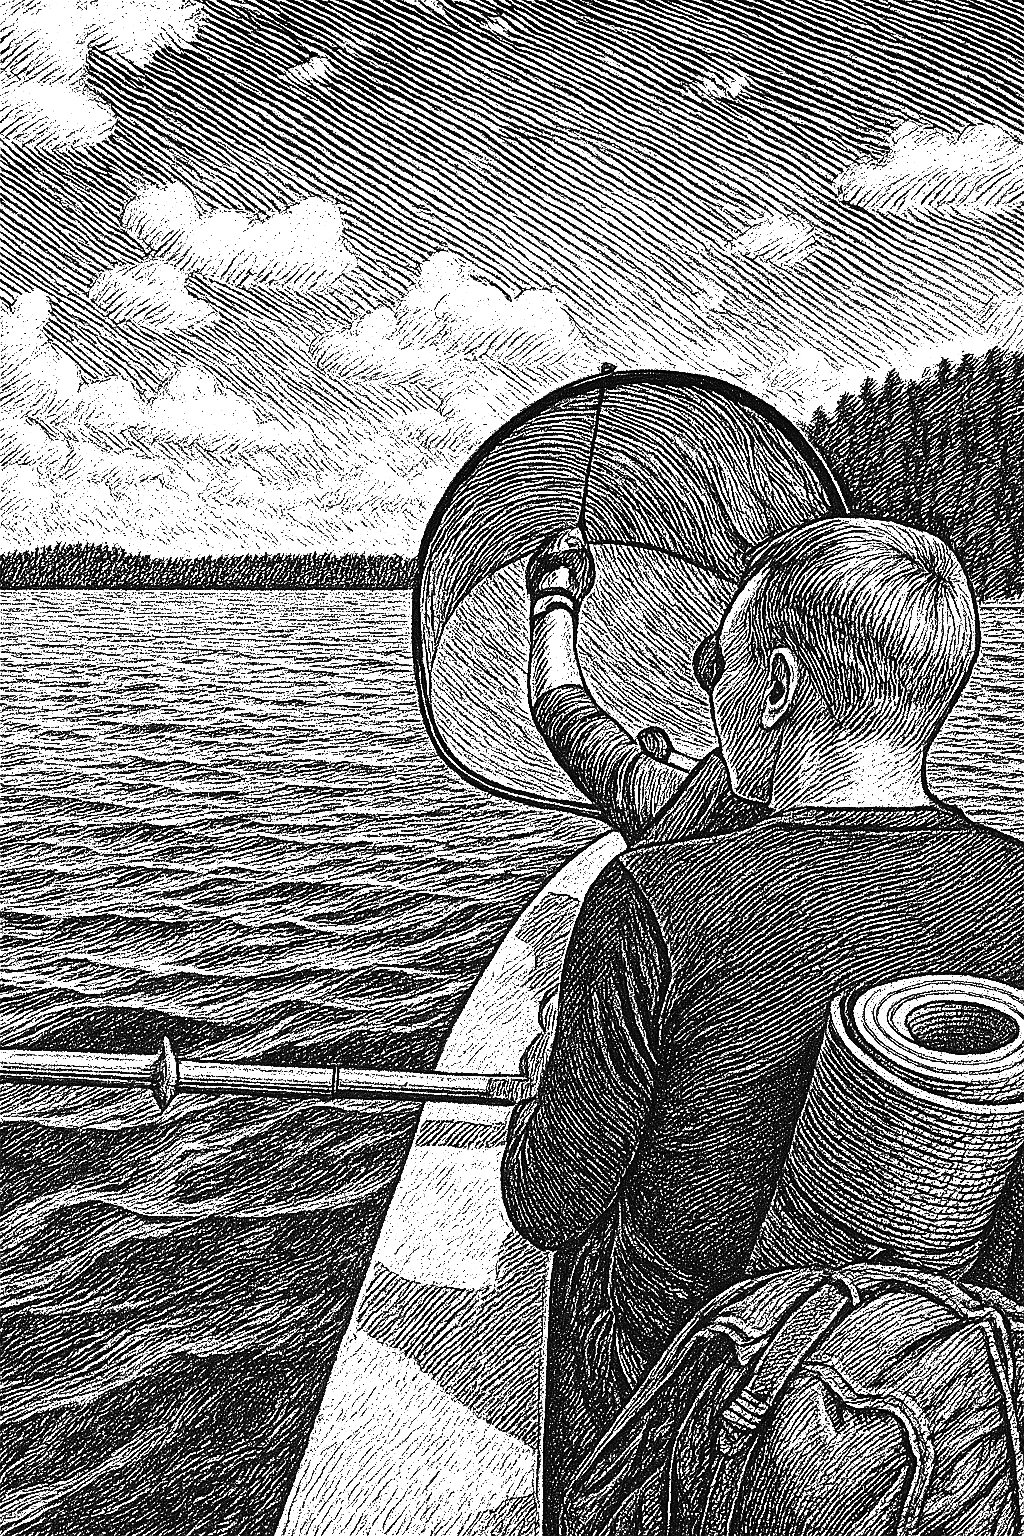
\includegraphics[width=0.95\linewidth]{16_1_parus}
	
	{\small\textit{...ветер стал усиливаться...}}
\end{minipage}


%	\begin{wrapfigure}[20]{r}{0.5\textwidth}
%%\begin{figure}[h]
%	\centering
%	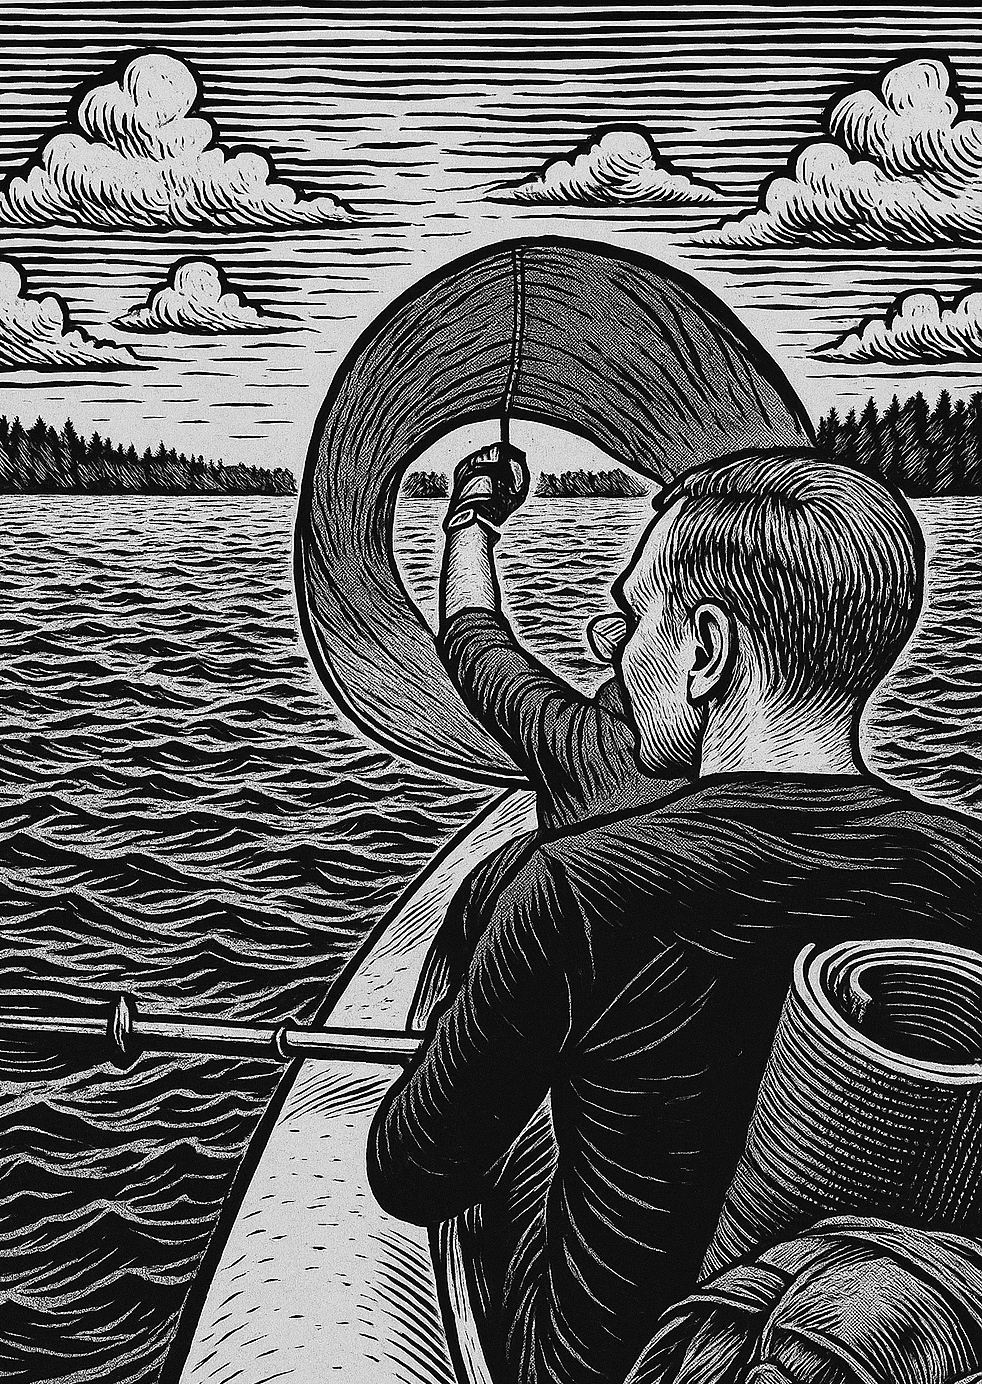
\includegraphics[width=0.5\textwidth]{8_1_new}
%	\caption{\small\textit{...ветер стал усиливаться...}}
%%\end{figure}
%	\end{wrapfigure}

%\renewcommand*{\thefootnote}{\arabic{footnote}}
%\setcounter{footnote}{0}
%Пашка разобрался с такелажем\footnote{Совокупность судовых снастей, в т.ч. для управления парусами\cite{МорскойСправочник}.}, привязал шкоты\footnote{Снасть бегучего такелажа, с помощью которой <...> оттягивают назад углы парусов\cite{МорскойСправочник}.} к~стальному тросу, приладил нижнюю часть паруса на~носовом шпангоуте и, наконец, полностью подготовившись, передал Адмиралу назад своё весло и взял в~руки шкоты, ловя ветер:

%\diagdash И\sdash и\sdash иха! 
%
%\diagdash ПОТАЩИЛО!!!\mdash Адмирал в полном восторге перестал грести веслом по\sdash байдарочному и взял его под мышку на манер руля.\mdash Погнали!!!
%
%Ветер дул, конечно, не~особо сильный, но этого было достаточно, чтобы дать им ход в парочку км/ч. Второй экипаж, тем временем, наконец\sdash то отчалил и догнал их:

\diagdash Пацаны, классно смотритесь!\mdash Серёге и Кире понравилась идея паруса.\mdash Но мы вас сделаем!\mdash они налегли на~вёсла и обошли адмиральскую байдарку вперёд.

\diagdash Нас обходят!\mdash Руслан схватился за весло.

\diagdash Ща мы их догоним в два весла плюс ветер! Держи парус, Паш!\mdash Адмирал подналёг на весло, и уже спустя пару минут они настигли второй экипаж.

Ветер стремительно тащил их на северо\sdash северо\sdash запад. Они так увлеклись парусом и гонкой, что позабыли про всё на~свете и уж конечно про исток речушки Сяпчи, соединявшей Сяпчозеро с Торосозером. Впрочем, Адмирал и не хотел идти по этой реке, надеясь пройти через канал, о~котором говорил команде с утра.

\diagdash Шу-у-урик! Там озеро кончилось!\mdash заявил Серёга, грёбший в почти полностью лежачем положении, вытащив и~растянув свои ноги на носу кириной байды.

\diagdash Куды рулим, тащ Адмирал?\mdash Киря рыскал по~курсу.

\diagdash Паш, сворачивай парус, надо свериться с GPS, да~и~ветер стих к концу озера.\mdash сказал Адмирал и, перехватив весло, достал навигатор, который висел у него на шее через плечо на длинной верёвке.\mdash Хм, пацаны, а~канал\sdash то правее! Мы его незаметно просквозили как\sdash то.\mdash обескуражено произнёс он, копаясь в навигаторе.

\diagdash Там не было ничего, Шурик!\mdash лёг на новый курс Замполит.

\diagdash Издалека может не разглядели, давай поближе подойдём!\mdash Адмирал был уверен, что канал на месте, поскольку, соотнеся пройденные каналы с увиденными ранее фотографиями в~Интернете, он сделал вывод, что то, что было изображено на фото, они ещё не прошли, а,~следовательно, канал в Торосозеро должен быть широким, глубоким и~ярко~выраженным. 

Спустя минут 10 эскадра вырулила к небольшим редким прибрежным зарослям\mdash из воды торчали тростинки. За~этими редкими зарослями начинался канал:

\diagdash А вот и он! Кирь, налегай!\mdash Серёга увидал канал, и~они с Замполитом первыми ворвались в его створ. Следом шёл адмиральский экипаж:

\diagdash Пацаны, снимайте на фото и видео! Где ещё такое увидите!\mdash Адмирал подруливал одной рукой веслом, а~второй умудрялся снимать видео на память, обозревая окрестности. 

Их маленькая эскадра вошла в канал шириной метров восемь и глубиной до полуметра. Он простирался ни много ни мало на километр вперёд. Борта его были выполнены из брёвен на~манер сруба, по берегам росла черника, брусника. Вид этого сооружения был ещё круче того, самого первого, которое они прошли вчера. Экипажи притормозили, ухватившись за~прибрежные заросли, и стали кушать чернику, росшую так вольготно и~обильно, что заросли этого кустарничка даже свисали прям с брёвен канала чуть не~до~самой воды. Наливные, синие почти до черноты, ягоды были крупными, спелыми, сочными:

\diagdash М-м-м! Вкуснятина!\mdash Серёга объедался с куста.\mdash Надо бы с собой набрать!

\diagdash Зачем? Я думаю её тут как грязи везде.\mdash ответил Адмирал.

\diagdash Не, в Москву с собой набрать!

\diagdash Ы-ы-ы! Скиснет пока довезёшь!

\diagdash Точно$\ldots$ Ну тогда на вечер, на компотик.

\diagdash Компотик\mdash эт хорошо! Я думаю в районе стоянки тоже будет черника.\mdash ответил Адмирал,\mdash Ну что, поели с куста? Поехали дальше!\mdash и~оттолкнулся от берега канала веслом.

Они плавно, почти не гребя, подходили к середине канала. Течение было слабым, но всё же было\mdash их жёлтые байдарки, плавно покачиваясь, скользили вперёд по водной глади, столь редко разрезаемой в этих местах сплавщиками. На нос замполитовой байды сели две стрекозы\mdash показатель экологической чистоты местности:

\diagdash Серёг! Снимай стрекоз! Вон, на носу!

\diagdash Точно! Красотища!\mdash тот перевёл фокус видео на~стрекоз.\mdash Благодать какая вокруг, пацаны!

\diagdash Да\sdash а\sdash а$\ldots$\mdash соглашался Адмирал.

Всем, надо полагать, нравилось подобное времяпрепровождение\mdash в спокойной тишине и наслаждении природой под ярким солнышком и лёгким ветерком. 

\diagdash Так, впереди мель и коряга!\mdash Серёга закончил с~видео и принялся выруливать левее по курсу. 

\diagdash Паш, не греби, я вырулю\mdash кинул вперёдсмотрящему Адмирал, и их маленькая эскадра успешно миновала коряги и мель посреди канала. Дальше ребята столь же безмятежно, как и до этого, потихоньку достигли конца канала.

\diagdash Тащ Адмирал, чё у нас дальше по плану?\mdash оживился Замполит.

\diagdash Дальше? Дальше ставим парус! Па\sdash а\sdash аш?

\diagdash Так точно, херр майор!\mdash Пашка развернул парус и~на~этот раз привязал его к веслу, используемому на манер мачты, чтобы не держать высоко руки со шкотами, что было утомительно. Конструкция вышла даже лучше прежней\mdash попутный ветер снова потащил их. 

\diagdash Шу-у-урик, ну а всё\sdash таки?\mdash не унимался Серёга.

\diagdash Дальше щас будет что\sdash то типа перекопа, короткого канала из озера Торос в озеро Мярандукса.\mdash вещал Адмирал.

\diagdash А если нет?

\diagdash А если нет, то попрёмся левее\mdash там короткая, на~один километр примерно, речка, соединяющая два озера! Всё как и~говорил с~утра, собственно.

Так, ловя ветер парусом и слегка отставая при этом от~кириной байды, адмиральский экипаж шёл вторым. Но это нравилось им гораздо больше гр{\'е}бли\mdash Паша вообще не грёб, а держал своё весло с расправленным парусом вертикально, Руслан подгребал, придавая им дополнительный импульс, а Адмирал только в основном выправлял курс веслом, корректируя вносимый ветром боковой дрейф.

Не желая петлять как перед прошлым каналом, Адмирал положил GPS прибор себе на колени и время от~времени сверял курс на следующий канал, идя под правым берегом озера Торос. Водная гладь была хороша, и, хотя озеро и было небольшим, всего около полутора квадратных километров по площади, ребятам нравился простор. Впереди их ждало озеро Мярандукса, такое же большое по площади, как и Сяпчозеро, на котором была их первая стоянка. 

Вскоре впереди замаячил ярко выраженный перешеек между озёрами, посреди которого виднелся проплыв. Сам перешеек был примерно метров 30\thinspace\nobreakdash---\thinspace 40 в ширину и~до~пяти метров в~высоту\mdash берега были крутыми, почти неприступными. Над небольшим коротким каналом, вид на~который вскоре открылся взору сплавщиков, лежало поперёк упавшее дерево, так что команда проплыла под ним, как под~мостом.

\diagdash Где пристанем?\mdash команде нетерпелось взобраться наверх.

\diagdash Давайте пройдём канал и зачалимся со стороны Мярандуксы\mdash там, я думаю, должен быть спуск к~воде, тут везде неудобно, сами видите!\mdash Адмиралу тоже очень хотелось осмотреть перешеек сверху, где он издали заприметил огромные сосны.

С обратной стороны перешейка берег оказался каменистым и крутым, но команде всё равно удалось пристать, надёжно закрепив чалки на деревьях. Адмирал~вытащил термос из гермы, снял штормовку, оставшись в~одной тельняшке, неторопливо прикурил сигарку и вскарабкался вместе с командой по обрыву наверх. Вид, открывшийся его взору, был шикарен\mdash прямо перед ними росла огроменная, в полтора обхвата, высоченная сосна с~раскидистой кроной и~старыми, причудливо изогнутыми ветвями. Ветер продувал узкий перешеек насквозь, ребята стояли под огромной сосной:

\diagdash Мы нашли Иггдрасиль!\mdash огласил Адмирал.

\diagdash Чего?\mdash спросил Серёга.

\diagdash Иггдрасиль! Мировое дерево в мифологии древних скандинавов! Корни его уходят в Хельхейм, царство мёртвых, ствол его пронзает Мидгард, мир людей, а верхушка достигает Асгарда, обители воинов\sdash асов.\mdash вещал тот. 

\begin{wrapfigure}[20]{r}{0.55\textwidth}
%\begin{figure}[h]
\centering
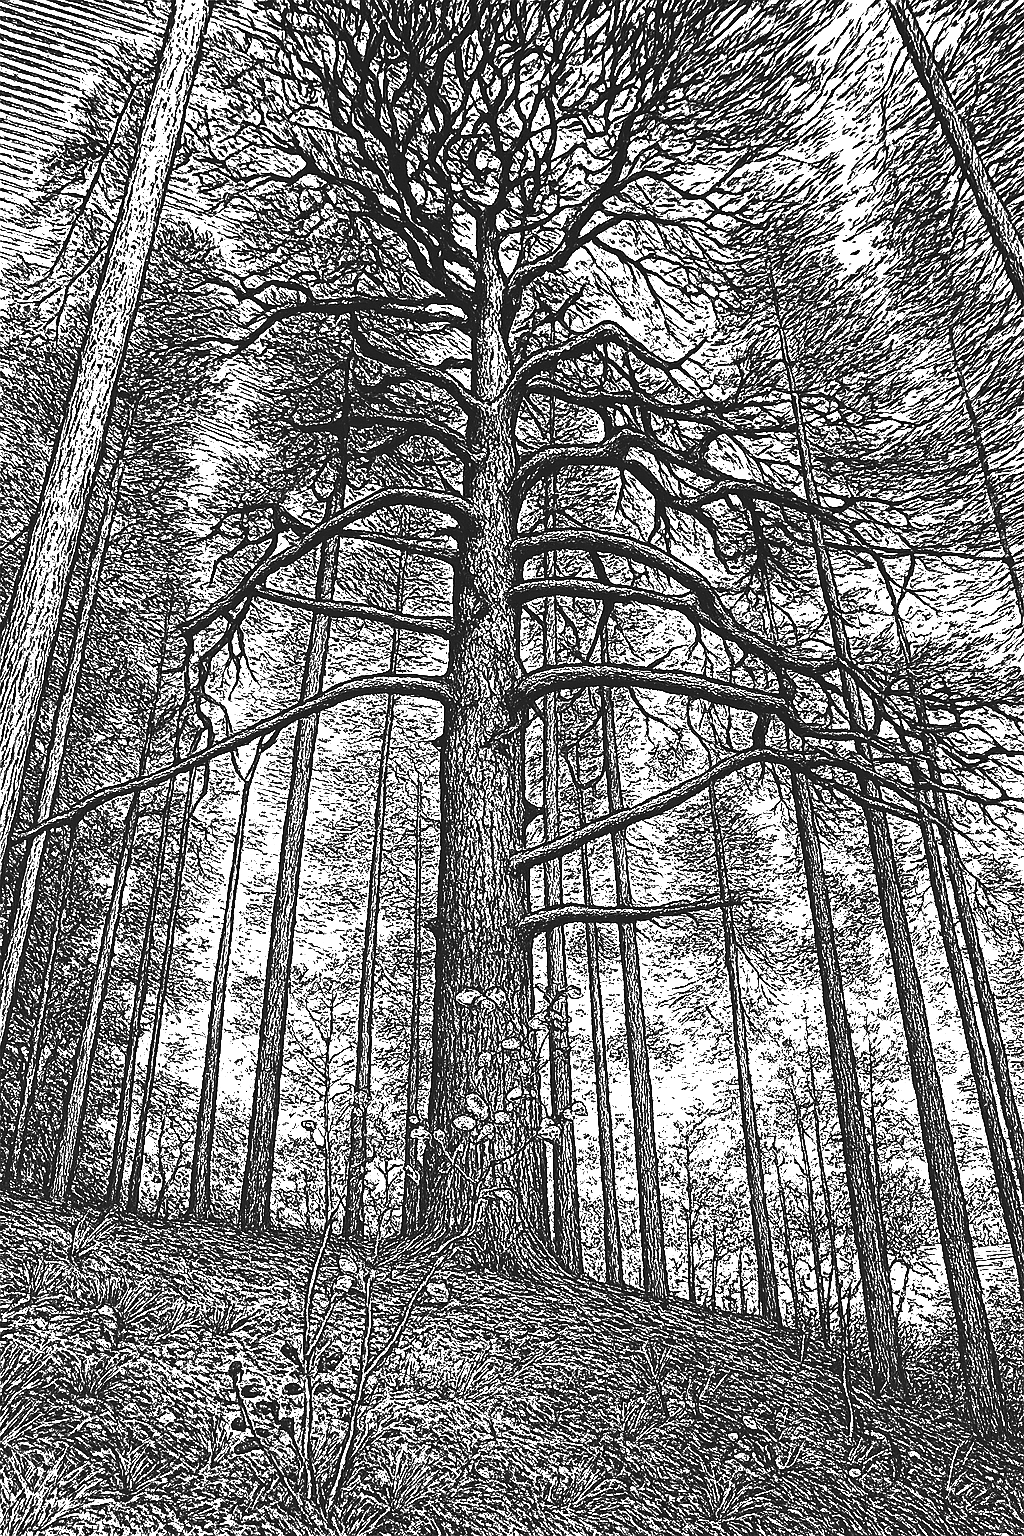
\includegraphics[width=0.55\textwidth]{17_2_tree}
\caption{\small\textit{...Мы нашли Иггдрасиль!...}}
%\end{figure}
\end{wrapfigure}
\diagdash Ваще похоже$\ldots$

\diagdash Шурик, там это, ясень был, у~скандинавов.\mdash сказал подошедший Киря.

\diagdash А у нас сосна будет! Она роднее как\sdash то. Мне всегда нравилась такая мифология\mdash древнегреческая и~древнеримская, потом древнескандинавская$\ldots$ Красиво они всё расписывали, черти!

\diagdash Да ты язычник?

\diagdash Это церковники христианские очернить чтобы придумали\mdash язычники, язычники, тьфу! У меня настольная книга была в школе\mdash <<Легенды и мифы Древней Греции и~Древнего Рима>>\cite{Кун}. Потом на~Скандинавию переключился$\ldots$ Красиво же! А не всё вот это <<ударили по левой щеке, подставь правую>>, тьфу! Ударили по одной щеке\mdash достал меч и~порубал обидчика нахрен, ёпрст!\mdash Адмирал выругался и~сплюнул.\mdash А~так~прав был дедушка Ленин: <<Религия есть  опиум для~народа!>>\cite{ЛенинОпиумДляНарода}. 

\diagdash Эк заворачиваешь! Ты лучше гляди, какие грибы растут!\mdash Серёга притащил два огромных подберёзовика, диаметром шляпки около двадцати пяти сантиметров.  

\diagdash Мощно, мощно! Ты смотри, ты смотри! Прям под ногами!\mdash Адмирал сделал шаг в сторону, нагнулся и поднял ещё один небольшой подберёзовик.\mdash Офигеть! Сегодня жарёху замутим вечером тогда из картошки с грибами!\mdash сказал он, увидав сколько грибов притащил Серёга. 

\diagdash Там дальше столик, костровище.\mdash сказал вернувшийся из разведки Паша и показал дальше вдоль по перешейку. Ребята пошли глянуть, но место никому не~понравилось, потому что перешеек насквозь продувался ветром, гулявшим между озёрами, к тому же на ночёвку становиться было ещё рано. 

Адмирал вернулся к <<Иггдрасилю>> и зачем\sdash то обнял это исполинское дерево, особняком стоявшее среди других, не менее высоких, но более молодых сосен. Ему было так хорошо, что хотелось навеки раствориться в красоте окружавшей его северной природы, которую он так любил. Он вдохнул аромат хвои и~смолы, исходивший от этой исполинской сосны. Этот запах, звучание которого глубоко засело в мозгу ещё с детства, со~времён велосипедных вылазок во владимирские леса, всегда будоражил в Шурике какие\sdash то приятные, но в то же время первобытные чувства, заставлял хоть на~секундочку очутиться в детстве$\ldots$ Сосны, тёплый запах смолы, мшаник, прибрежные камни и песочек, лёгкий ветер и иссиня\sdash синее августовское небо уносили Шурика в его какую\sdash то другую реальность. На Землю заставили спуститься лишь голоса~команды:

\diagdash Ну что, тащ Адмирал, идём дальше?\mdash Серёга и~Киря собрали грибы в пакетик на вечер и готовы были спускаться к байдаркам.

\diagdash Да, щас пойдём.\mdash Шурику не хотелось уходить от <<Иггдрасиля>>, он всё ещё стоял, прислонившись к тому. Паша и Руслан пошли вниз к байдаркам, пора было отчаливать.

Все аккуратно спустились с перешейка к своим кораблям, уселись, отчалили. Адмирал отходил от берега кормой, совершая разворот на $180\degree$ по курсу через берег, чтобы ещё раз окинуть взором шикарной красоты место, которое они покидали. 

\diagdash Тащ Адмирал, впереди просто Атлантика! Куда идём?\mdash поинтересовался Замполит.

%\renewcommand*{\thefootnote}{\arabic{footnote}}
\renewcommand*{\thefootnote}{\fnsymbol{footnote}}
\setcounter{footnote}{0}
\diagdash Кильватерной\footnote{Кильватер (гол. kielwater)\mdash строй кораблей <$\dots$> идущих друг за~другом в~одной линии <$\dots$>. Идти в~кильватер\mdash значит идти вслед за~впереди идущим судном\cite{МорскойСправочник}.} колонной за мной! Держим курс по~спутниковой навигации!\mdash отозвался Адмирал.\mdash Впереди мыс виднеется слева\mdash правим на него, там должен открыться простор озера Мярандукса во всей красе!

\diagdash Мярандукса,\mdash медленно произнёс Руслан.\mdash прикольное название!

\diagdash Ну да, тут деревня была раньше на правом берегу с~таким же названием. Или у озера такое же название, как у~деревни, поди разбери теперь. На месте деревни уже ничего нет, так что пойдём тут, под левым берегом.\mdash заключил Адмирал.

\diagdash Сань, ветер не очень, парус не ставлю?\mdash Пашке, естественно, очень понравилось сидеть и рулить парусом, не~гребя. Есть что\sdash то завораживающее в управлении парусами, кто бы что ни говорил! Недаром этим гениальным древнейшим изобретением человечество пользуется и~по~сей~день.

%\renewcommand*{\thefootnote}{\arabic{footnote}}
\renewcommand*{\thefootnote}{\fnsymbol{footnote}}
\setcounter{footnote}{0}
\diagdash Ага, ветер почему\sdash то почти встречный, хотя на~прошлом озере был попутный. В лавировку\footnote{Продвижение парусного судна к цели, расположенной с наветренной стороны, в бейдевинд переменными галсами. Галс (голл. Hals)\mdash курс судна относительно ветра\cite{МорскойСправочник}.} с таким парусом не пойдёшь$\ldots$\mdash сказал Адмирал и погрузился в~свои мысли о парусе. Ему безумно хотелось когда\sdash нибудь выйти да даже хоть и на такое озеро, но под более менее приличным парусом, квадратов на 4 или 5 площади. Юрич на работе всё убеждал его сделать парусное вооружение на~байдарку, но ему хотелось собрать непременно парусный катамаран из двух байд\sdash трёшек$\ldots$

\vspace{0.5cm}
$\ldots$Вскоре ребята достигли мыса\mdash им открылся вид на~остальной простор озера, который не был виден за мысом до этого момента. У всех дух перехватило от простора и~красотищи:

\diagdash Шу-у-рик! Это прям ух!\mdash не то с восторгом, не то маленько со страхом сказал Серёга.

\diagdash Ух-ух!\mdash передразнил Адмирал.\mdash Правим во-о-он на те островки, обойдем их справа.\mdash провёл он краткий инструктаж.

\diagdash Каков расчёт?\mdash осведомился Замполит.

\diagdash Править к левому берегу, там есть один мыс характерный, сто процентов там есть хорошая стоянка. Под~правым берегом высоковато, не хочется там идти$\ldots$

\diagdash Ну лад\'{ы}! Кто быстрее?\mdash и Замполит принялся лопатить веслом.

\diagdash Врёшь! Не возьмёшь! У нас три весла! А ну, парни, сделаем этого выскочку!\mdash Адмирал скомандовал полный вперёд, и они в режиме гонки дошли до~скопления маленьких островов посреди Мярандуксы. Обойти Замполита не~вышло\mdash его двушка была менее загружена и имела меньшую осадку, нежели чем адмиральская трёшка. 

Парни шли в полукилометре от берега, временами было не~очень комфортно осознавать себя вдали от земли, но это чувство быстро проходило за греблей. Наконец, они достигли последнего маленького островка среди этого небольшого архипелага и прошли совсем рядом с ним:

\diagdash Шу-у-рик, заберёмся?\mdash спросил Серёга.

\diagdash Нафига?\mdash парировал Адмирал.

\diagdash Ну просто, интересно.

\diagdash Там заросли такие, да и остров настолько мелкий, что стоянку на нём не устроить, пошли дальше.

\diagdash А чего на тот мыс большой залезать не стали?\mdash спросил Серёга, обернувшись и посмотрев назад.

\diagdash Там кладбище было от этой исчезнувшей деревни Мярандукса, урочище которой прошли по правому берегу. Многие не знают и встают там лагерем, место\sdash то красивое. А~потом кресты старые находят чуть поодаль$\ldots$ Так что мы дальше пойдём.\mdash сообщил Адмирал подчерпнутые из~отчётов по~маршруту сведения.

В районе следующего острова они скорректировали курс эскадры, потому что Адмирал чуть отвлёкся от~навигатора и перепутал на какой мыс впереди править\mdash по итогам оказалось, что на ближний, около которого вскоре издалека показалась то\sdash о\sdash оненькая полосочка песка, пляж.

\diagdash А? Что я вижу? Пляжик, тащ Адмирал!!!\mdash Замполит приободрился и налёг на весло.

\diagdash А то?\mdash подмигнул тому Адмирал.\mdash Я плохой стоянки не посоветую!

Они бодро налегли на вёсла, держа курс на выбранный мыс. Однако по мере приближения к пляжу Адмирал понял, что не всё так радужно\mdash пляж был в стороне от~мыса, тропинки между ними не просматривалось. Вскоре эскадра зашла в~маленький заливчик, заканчивающийся пляжиком, и~выбросилась байдарками на~песок, ребята вылезли. Водичка в~озере бодрила.

\diagdash Так! Матросы охраняют байды, поскольку чалиться тут особо не за что. Паш, Кирь\mdash за мной!\mdash и они пошли пробираться через заросли к возвышенности на мысу, где по адмиральским предположениям должно было быть стояночное место.

\diagdash Шурик, куда мы прёмся? Болотина какая\sdash то!\mdash изрёк Замполит, заплетаясь ногами и стараясь не грохнуться в чёрную мокрую грязищу. От их поступи в~размокшем грунте раздавалось чавканье.

\diagdash Не гунди, вон уже подъём начинается!\mdash Адмиралу тоже было тяжко, но ему больно хотелось поглядеть на~стоянку. 

Вскоре они взобрались по подъёму от болотины наверх. Адмирал чуть не ахнул\mdash рай на Земле! Взору~разведчиков открылась гряда шириной метров 15, посередине которой было ровное место, устланное сосновыми иголками, а~по~бокам росли могучие высокие сосны. Чуть поодаль виднелся стол, две скамейки и костровище с~большими камнями и брёвнами вокруг. Прямо по~краям поляны росла черника. Словом, место покорило их~с~первого взгляда. Киря рванул к~костровищу:

\diagdash Тащ Адмирал, остаёмся!

\diagdash А то! Иди забей нам место под~палатку на~мысу\mdash там по\sdash моему кошернее всего\mdash в окружении сосен и площадка ровная.\mdash Адмирал намётанным глазом уже прикинул как и где они поставят лагерь, оценил и~расположение сосен у стола\mdash они позволят натянуть тент от дождя прямо над столом и~скамейками. 

Паша, тем временем, походил по мысу в поисках <<рыбного места>> и вернулся кисловатый:

\diagdash Рыбачить особо негде! Везде высокий берег, капец. Только вот тут что ли, у костра, спуск более менее!

\diagdash Ну что поделать, значит так. Место\sdash то в целом\mdash вообще кайф!

\diagdash Это да$\ldots$ Ладно, чё по разгрузке? Таскать далеко. Давай сюда байды подведем, под обрыв к костровищу? 

Адмирал сходил посмотрел обрыв, оценил перспективы и понял, что не вариант\mdash глубина у берега не позволяла стоять в воде, так что вещи пришлось бы кидать на берег:

\diagdash Полюбас тут кто\sdash нибудь грохнется или чё\sdash нить утопит, пока разгружаться будем. Пойдём лучше через болотину перетаскаем\mdash каждому всего\sdash то раза по два придется сходить.\mdash Адмирал пошёл обратно к спуску в~болотину, позвав с~собой Замполита.

\diagdash Эх\sdash х!\mdash Паша обречённо вздохнул и пошёл за ними.

Издалека, пробираясь по чавкающей под ногами почве, Адмирал крикнул Серёге и Руслану, чтоб те начинали разгружаться. Вскоре команда разгрузила байды, затащила их с пляжика в лесочек и перевернула кверху днищем. Вещмешки и гермы таскали наверх с максимальной нагрузкой, чтобы минимизировать количество проходов по~болотине: 

\diagdash Куда ставить\sdash то?\mdash Замполит по\sdash богатырски тащил на двух согнутых в локте руках по вещмешку на лямках, а~сверху лежала продуктовая герма.

\diagdash К костровищу давай, около стола сваливай\mdash там будет хозчасть.\mdash распорядился Адмирал, а сам, тем временем, притащил свою герму и стал ставить их с~Замполитом палатку\mdash ему хотелось быстрее развернуть лагерь и пойти искупаться, пока солнце ещё грело и светило на полную катушку.

Серёга, Руслан и Паша поставили свои палатки дальше от костра, в ряд вдоль по мысу, сразу за адмиральской палаткой, и~тоже включились в~хозяйствование. Паша решил забросить удочку, что называется, на казус, поскольку хорошего улова не ожидал, а Адмирал с Замполитом побежали скорее купаться. Адмирал выбрал банное местечко на камнях чуть поодаль на пляжике, разложил там своё полотенце и банные принадлежности, а потом вошёл в воду: 

\diagdash Ух\sdash х\sdash х! Водичка\sdash то\mdash огонь просто!!! Киря, не~отставай!\mdash заорал он тому и выбежал на~берег, стал намыливаться.

\diagdash Шурик, ты просто морж!!! Вода ледянющая!\mdash Киря зашёл по коленочки и обтёрся водой.

\diagdash Фигня! Щас привыкнешь!\mdash Шурик, весь намылившись, растёрся мочалкой и стал потихоньку входить в воду ополоснуться. Дно на этом пляжике было песчаным, с редкими камнями, и относительно медленно уходило на~глубину, так что надо было пройти метров двадцать, чтобы иметь возможность полностью окунуться. Наконец, он вышел на глубину и посмотрел вдаль. На~горизонте за~рябью озера виднелась гора Ундойвара с~геодезическим пунктом на~вершине.  

Шурик стоял по~пояс в~холодной воде и~собирался с~мыслями. Перед ним расстилалось зелёное море карельского леса и~синее море Мярандуксы. Ему почему\sdash то казалось, что он совершает чуть не~священнодейство, окунаясь в~это холодное озеро. Наконец, он собрал волю в~кулак, продышался три раза полными лёгкими и~нырнул на~глубину. Как и~всегда в~таких случаях, звуки приглушились, размытое бульканье заполнило слух. Он~плыл под~водой, усиленно работая руками и~ногами. Время как бы замерло в его сознании, а секунды, проведённые под водой, казались вечностью. Наконец, он с~силой вырвался из~водной глади вверх на~поверхность, заорав:

\diagdash А-А-А-А-А!!! Хорошо!!!
\nopagebreak

Потом Шурик выплыл к берегу и вышел будто бы обновлённым, так рисовалось ему во взбудораженном холодом сознании.

\diagdash Киря!!! Давай!!! 

\diagdash Ага! Хоп!\mdash Киря тоже продышался и нырнул.\mdash Ой\sdash й\sdash й хорошо!!!\mdash вынырнув, громко заорал он, размахивая при этом руками.\mdash Ой\sdash й\sdash й хорошо\sdash о\sdash о!!!

\diagdash А я тебе о чём?

Киря быстренько растёрся полотенцем, выскочив на~берег, и аккуратно поскакал через болотину обратно к~лагерю, а Шурик остался. Он в темпе постирался и~решил искупаться ещё разок. Но~перед этим прошёлся по~пляжику и~сорвал веточку растущей прямо тут~же зелёным пушистым ковром черники и~стал есть, отрывая ягоды губами. 

{
\setlength{\belowcaptionskip}{-5mm}
\begin{figure}[h]
\centering
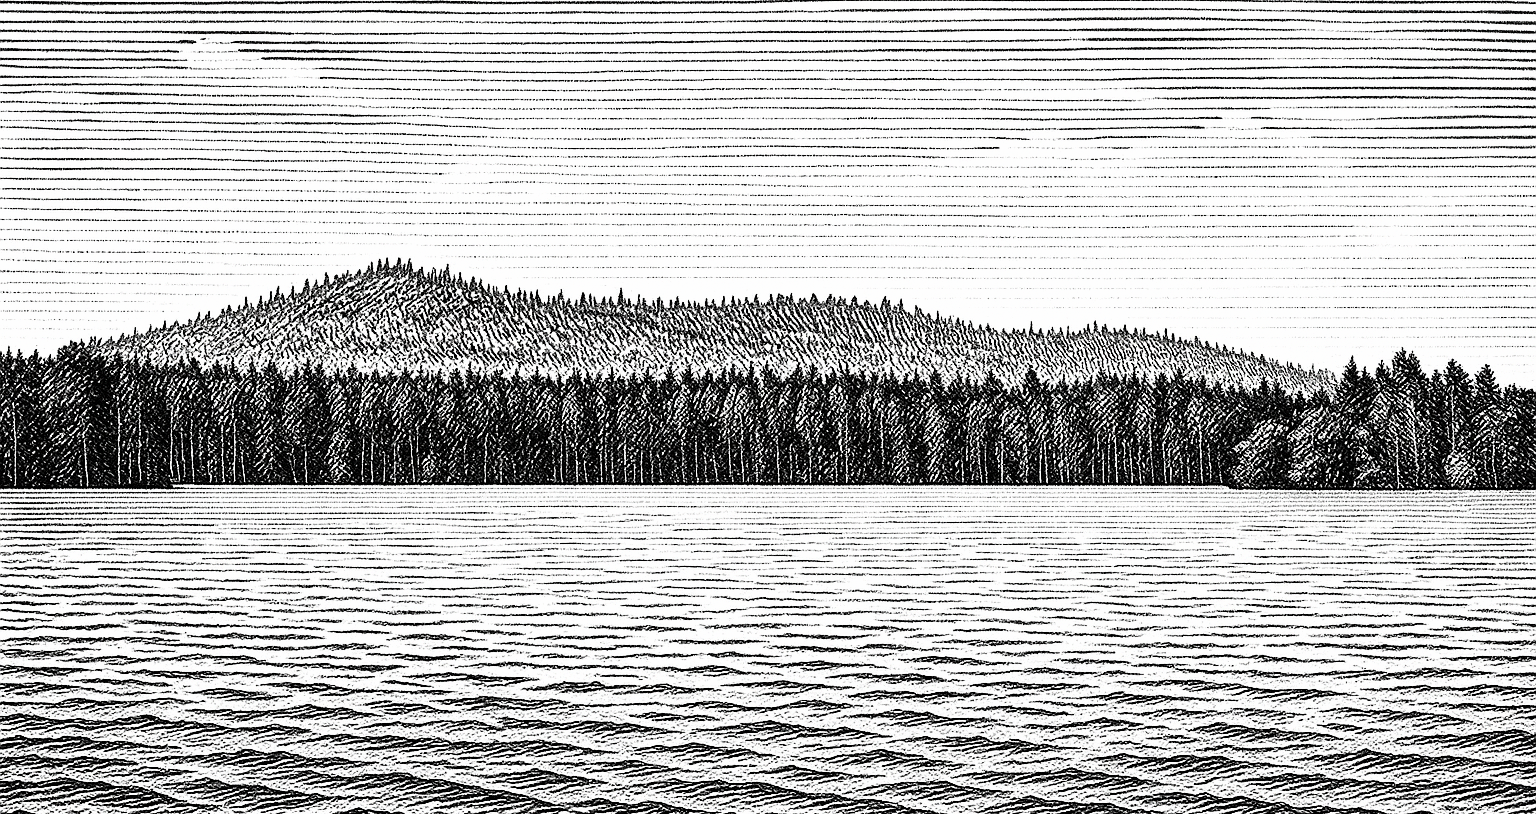
\includegraphics[width=1.0\textwidth]{18_mountain}
\caption{\small\textit{...На~горизонте виднелась гора Ундойвара...}}
\end{figure}

Он присел на песочек и~посмотрел вдаль на гору Ундойвара. До неё по~прямой было около четырёх километров, а по тропкам, если они есть, все шесть. Если предпринять попытку восхождения, то~надо оставаться на~днёвку, а дневать было ещё рановато, он это понимал, хоть место и было располагающим. Идею о восхождении он оставил на следующее прохождение этого маршрута, в~котором он уже совсем не~сомневался\mdash Карелия захватила его душу и сознание с первого взгляда$\ldots$ 
}

\vspace{0.1cm}
$\ldots$Очнувшись, он доел чернику и пошёл окунаться ещё раз. Вода перестала казаться ледяной, он привык к~холоду и~проплыл ещё прилично, пока, наконец, не ощутил ледяное дыхание глубины озера. Адмирал вышел на песочек и~растёрся полотенцем\mdash ему было так хорошо, что хотелось не то что петь, хотелось просто орать в сине\sdash зелёную даль. Ему вдруг вспомнился сегодняшний Иггдрасиль и~разговоры о мифах и~сказаниях. Он встал, выпрямился, закинул голову в небу и~расставил руки в стороны. В это время солнце, на~несколько минут скрывшееся за налетевшим облаком, вновь озарило всё своими оранжевыми вечерними лучами. Шурик простоял так пару минут, наслаждаясь этим состоянием, толком объяснить которое он был не в силах. Наконец, он ещё раз бросил взгляд на гору на горизонте и,~собрав вещи, пошёл наверх в лагерь.

Паша, тем временем, уже почистил часть грибов, пока ребята купались:

\diagdash Так, Сань, чё конкретно с грибами делаем? Варим?% Жарим?

\diagdash Ну\sdash у\sdash у, давай сначала отварим, а потом зажарим с~лучком?

\diagdash Ага! И картоху надо!\mdash решили делать грибную жарёху с картошкой.

\diagdash Ща переоденусь и картоху почищу тогда, и на суп надо почистить всё.\mdash Адмирал присел в палатке, мигом утеплился и пошёл к костру\mdash он был на мощнейшем эмоциональном подъёме после купания.

Серёга, отдав Паше инициативу чистки грибов, пошёл в лес за черникой, очень уж ему она понравилась. Из~леса раздавались его восторженные возгласы по поводу количества черники. Адмирал, положительно оценив как команда начала налаживать прикостровой быт, развёл костерок, распотрошил мешки, достал провизию, прикинул как и что будет готовить, открыл свой складной ножик и~принялся за картошку.

Тут зазвонили колокольчики, привязанные на пашкину удочку. Тот мигом сорвался от стола к берегу и вытащил приличную рыбину, бьющуюся на леске:

\diagdash Вау, первая пошла!

%\diagdash Класс! Дай сфоткаю!\mdash Адмирал вытер руки от~картошки об~штаны и достал свою зеркалочку запечатлеть добычу.\mdash По красоте, вообще!!! Так, надо бы эц\sdash самое!

\diagdash Класс! Дай сфоткаю!\mdash Адмирал вытер руки об~свои камуфляжные штаны и~достал свою зеркалочку запечатлеть добычу.\mdash По красоте, вообще!!! Так, надо бы эц\sdash самое!

\diagdash Точняк! Где апельсины?!\mdash моментально нарисовался Замполит.

\diagdash Хоп-па! Ещё одна!\mdash Паша вытащил ещё одну рыбину.

\diagdash Огонь, дело спорится!\mdash Замполит подключил музыкальную колонку и нарезал закуску.

\diagdash Мужики, она просто на щепки берёт!!!\mdash Паша вытащил ещё одну рыбку. Все они были примерно сантиметров по 25\thinspace\nobreakdash---\thinspace 30.

\diagdash Отлично! Варим уху, однозначно!!!\mdash Адмирал уже почистил картоху, морковку, лук.\mdash Тащ Замполит, апельсин нарезал?

\diagdash А то!\mdash Киря разлил. Серёга как раз подошёл с~полным пехотным котелком черники.\mdash Ого, гляди чё тут мой матрос надыбал!

%\renewcommand*{\thefootnote}{\arabic{footnote}}
\renewcommand*{\thefootnote}{\fnsymbol{footnote}}
\setcounter{footnote}{0}
\diagdash Так, пацаны!\mdash Адмирал поднял железную кружку с ромом и взял дольку апельсина.\mdash SKÅL{\footnote{Древнескандинавский тост <<За здоровье>>, произносится как <<скол>>}}!

\diagdash {\Large SKÅ-Å-ÅL!!!}\mdash бешеным ором отозвалась команда и осушила железные кубки.

\diagdash Не-не-не, пацаны, не <<скол>>, а это, как его$\ldots$ Кампай! Во!\mdash тоненьким голоском спародировал Пашка. 

\diagdash Это чё?\mdash Адмирал, возмутившись, закусил апельсинчиком.

%\begin{wrapfigure}[12]{r}{0.5\textwidth}
%%\begin{figure}[h]
%	\centering
%	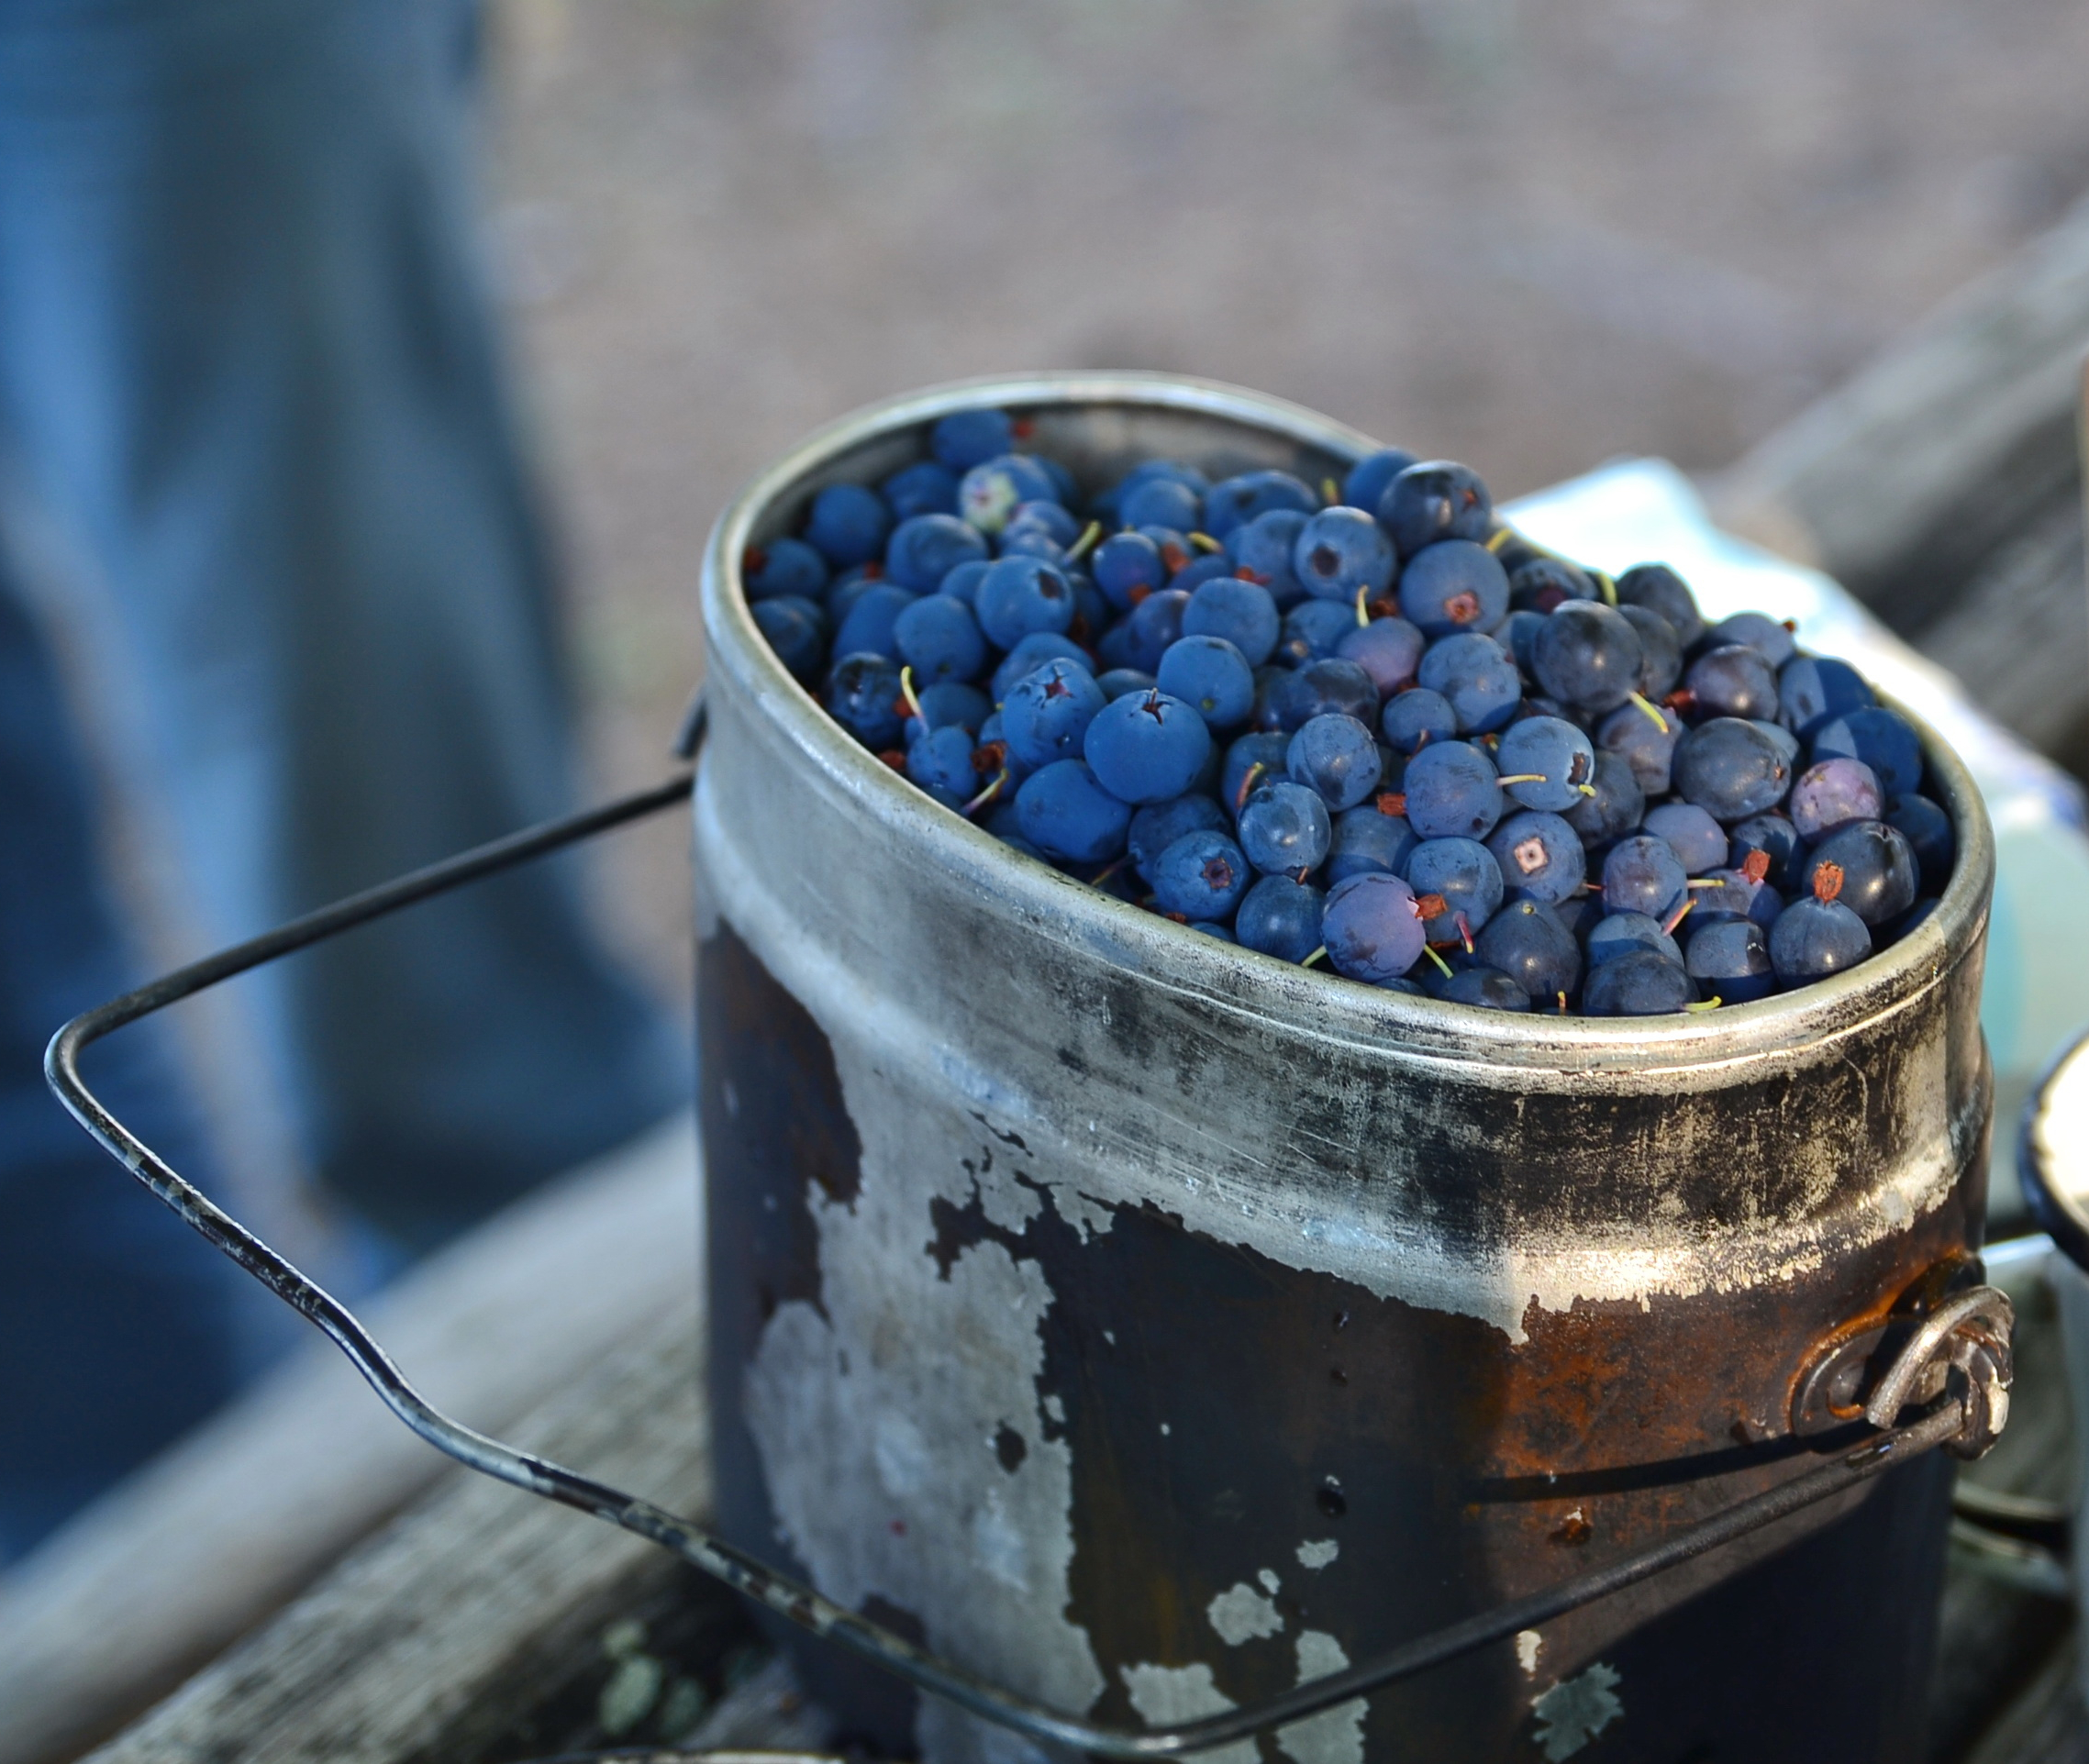
\includegraphics[width=0.5\textwidth]{8_4}
%	\caption{\small\textit{...Полный котелок черники...}}
%%\end{figure}
%\end{wrapfigure}
%\diagdash У-у-у! Темнота! Это из~этого, из~японских мультов, короче, у~меня дети смотрели там чёта такое.\mdash просветил всех Паша.\mdash Давайте ещё по~одной?
%
%\diagdash Подтверждаю, есть такое в аниме.\mdash Замполит разливал ещё.

%\noindent
%\begin{minipage}{0.45\textwidth}
%	\setlength{\parindent}{1.0cm}  % Включаем красную строку
%	\setlength{\parskip}{0.25cm}     % Межабзацный отступ, как в основном тексте
%	
%	\diagdash У-у-у! Темнота! Это из~этого, из~японских мультов, короче, у~меня дети смотрели там чёта такое.\mdash просветил всех Паша.\mdash Давайте ещё по~одной?
%	
%	\diagdash Подтверждаю, есть такое в аниме.\mdash Замполит разливал ещё.
%	\end{minipage}\hfill
%	\begin{minipage}{0.45\textwidth}
%	\centering
%%	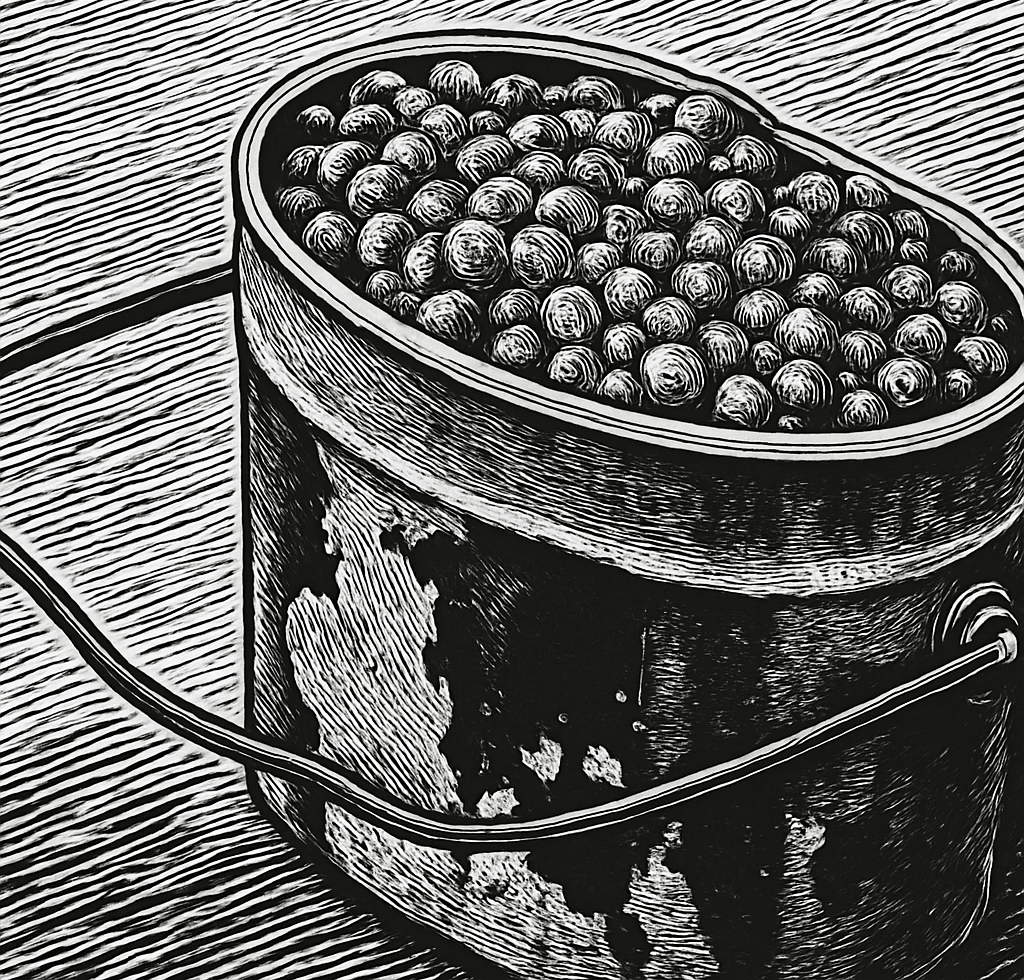
\includegraphics[width=\linewidth]{8_4_new5}
%	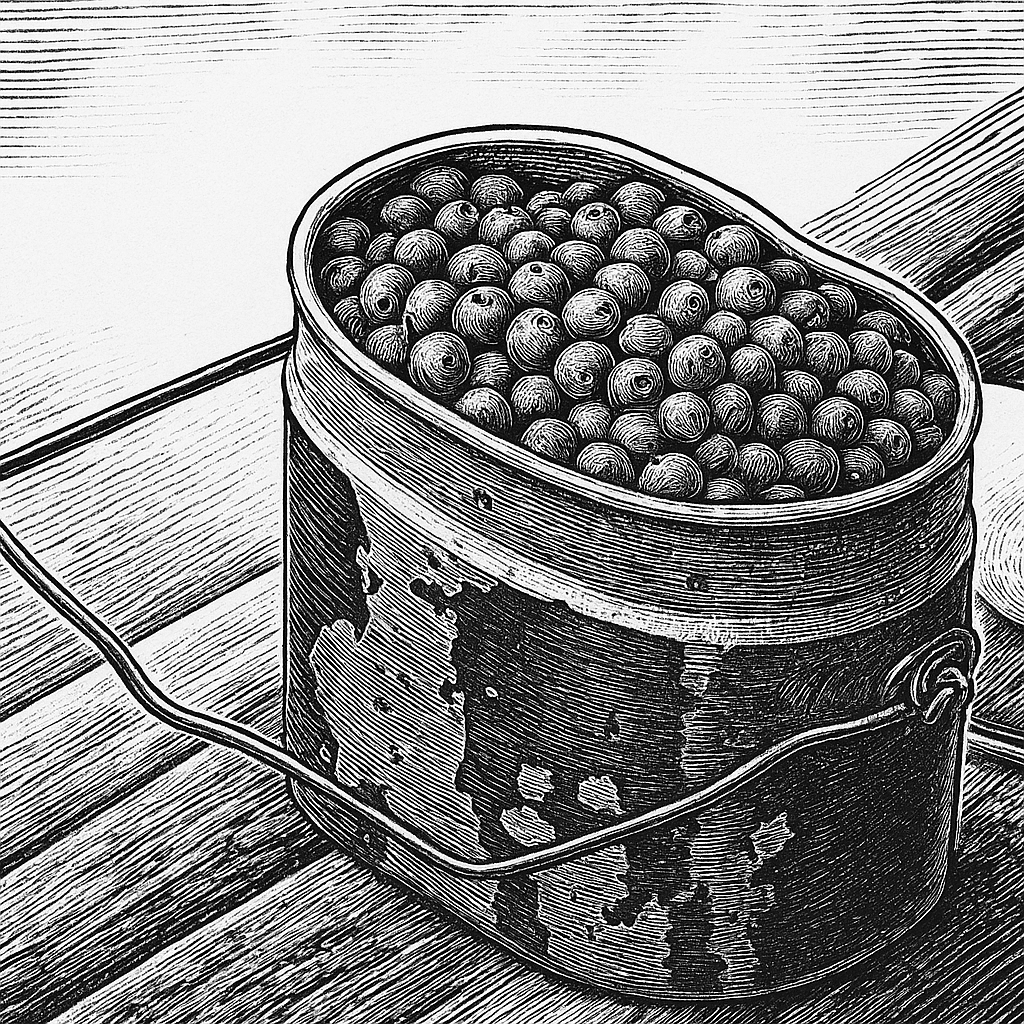
\includegraphics[width=\linewidth]{11_gpt}
%	
%	{\small\textit{...Полный котелок черники...}}
%\end{minipage}

\begin{wrapfigure}[11]{r}{0.45\textwidth}
	%\begin{figure}[h]
	\centering
	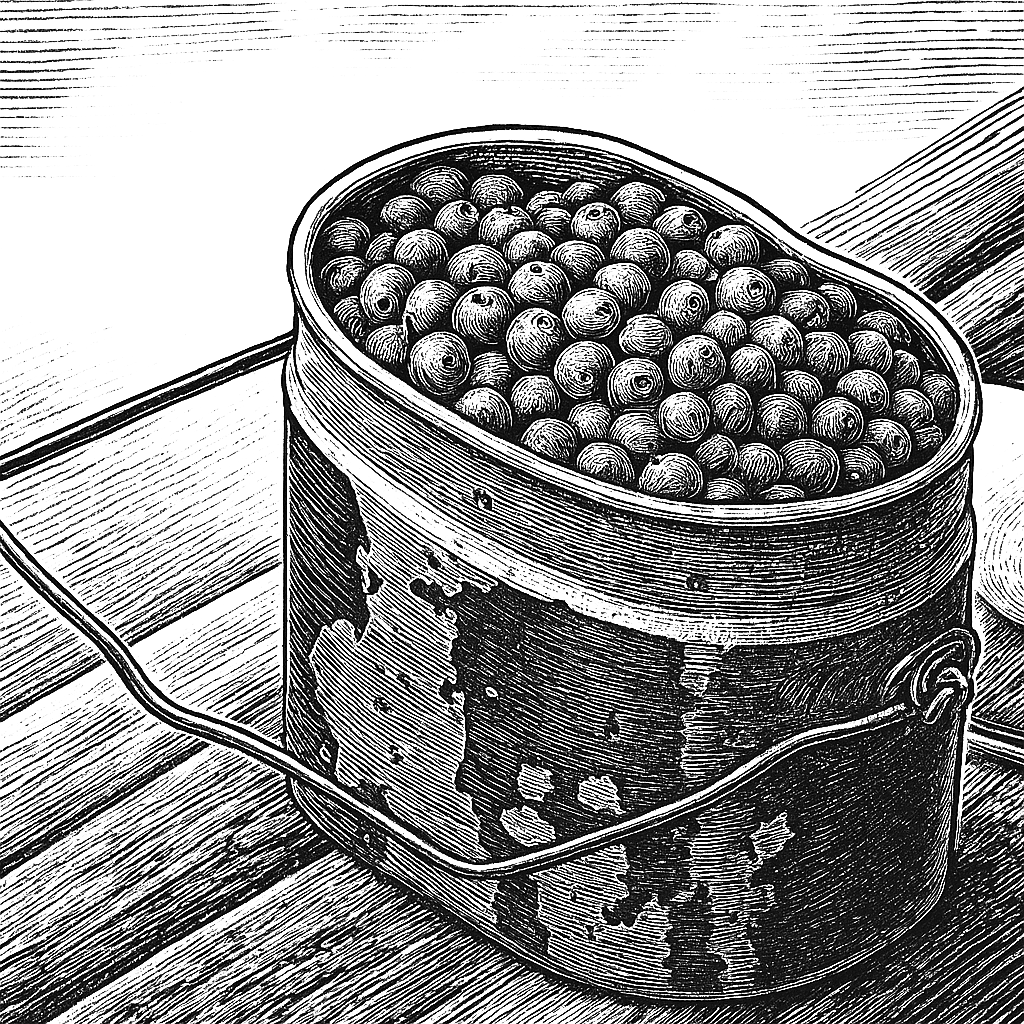
\includegraphics[width=0.45\textwidth]{19_1_blueberry}
	\caption{\small\textit{...Полный котелок черники...}}
	%\end{figure}
\end{wrapfigure}


\diagdash Не, парни, только троекратное <<УРА>> или <<SKÅL>>!\mdash Адмирал взял дольку апельсинчика.

%\diagdash Не, парни, только расово\sdash чистое троекратное <<УРА>> или <<SKÅL>>!\mdash Адмирал взял апельсинчик.

\diagdash Пофиг, будем!\mdash лес железных кубков поднялся.

\diagdash Кампай!

\diagdash SKÅL! Ну тебя с этим <<кампаем>>! Давай компотик варить!\mdash Адмирал попробовал спелую чернику.

\diagdash Кампай!\mdash не унимался Паша.

На берегу зазвенели колокольчики.

\diagdash Беги скорее, кампай, блин!

Пашка бросил кружку и сорвался к удочке. Подсечка и~спустя мгновение на леске красовалась очередная сверкающая серебряной чешуёй и красными плавниками рыбина:

\diagdash Офигеть, по одной штуке раз в пять минут! Уха будет знатная!

Серёга, тем временем, тоже соблазнился возможностью пойти искупаться и быстренько реализовал это, вернувшись с~пляжа бодрячком. Потом они с Русланом поставили на~огонь большой котелок наварить компота. Адмирал, продолжая возиться с грибами, зажарил картошку с~луком на~маленькой алюминиевой сковородочке, которую приобрёл взамен старой тяжёлой чугунной. 

\diagdash Колокольчики!!!

Пашка опять сорвался от стола к берегу\mdash ещё одна рыбина стала добычей. Улов уже достиг внушительных размеров\mdash большой полиэтиленовый пакет с водой был полон плотвы и краснопёрок. За час, чистя рыбу и постоянно отвлекаясь на колокольчики, Паша легко наловил на уху.

Шурик кайфовал от происходящего, наслаждаясь моментом. Ему нравилось решительно всё, как проходил этот вечер\mdash и стоянка, и своя команда, и стол, и, разумеется, великолепие природы. Он включил через колоночку:

%\newpage
\vspace{0.2cm}
\noindent\textit{%
	\hspace*{1.5cm}А у нас у ворот да зелёнай сад да расцвитал,\\
	\hspace*{1.5cm}Да о-о-ох, да ляли лёли расцвитал.\\
	\hspace*{1.5cm}Да ты двор чистый засиял ал{\'ы}ми цв{\'и}тами,\\
	\hspace*{1.5cm}Да о-о-ох, да ляли лёли цв{\'и}тами.\\
	\\
	\hspace*{1.5cm}А в том с{\'а}ду да берёзушка стоял{\'а}\\
	\hspace*{1.5cm}Да о-о-ох, да ляли лёли стоял{\'а}.\\
	\hspace*{1.5cm}Да по берёзушке перепёлушка литал{\'а}\\
	\hspace*{1.5cm}Да о-о-ох, да ляли лёли летал{\'а}$\ldots$
}
\vspace{0.2cm}

\diagdash Шурик, что это?\mdash народ был под впечатлением.

\diagdash Эт современная обработка русской народной песни, шо таки вам не нравится? Как по мне\mdash трогает струны души!\mdash Адмирал суетился с готовкой и наслаждался девичим вокалом.

\diagdash Весьма, я бы сказал$\ldots$ \mdash Замполит разлил ещё.

Паша доканчивал чистку рыбы, руки по локоть были в~блестящей чешуе:

\diagdash А у нас же там ещё сало!!!\mdash вспомнил он.\mdash Сань, где оно? Доставай!

\diagdash Вон в тряпочке лежит, разверни!

\diagdash Тэк-с, я бутеры с салом и лучком накручу!

\diagdash Слушай, офигеть улов! А ты говорил место не очень, место не очень$\ldots$

\diagdash Да кто ж знал?! Так, у всех налито?\mdash Паша поднял в одной руке кубок, а в другой бутер с салом.

\diagdash SKÅL!\mdash проорала команда.

\diagdash Кампай!\mdash тоненьким голоском спародировал Пашка.

\diagdash Фу ты ну ты со своим <<кампаем>>!

\diagdash Ы-ы-ы!!!

Веселье начало стремительно закручиваться. Адмирал закончил жарить отваренные грибы и смешал их с~картошечкой\mdash вышло прелестно. Паша наконец дочистил рыбу, Серёга наварил компотика. Руслан осваивался в~походной остановке, Киря сел к столу и наворачивал поспевшую картоху с грибами:

\diagdash Шурик, оч вкусно! Закусон мировой, идёт просто кайфец!

\diagdash Да ваще! Сделай музон погромче!!!

\diagdash Угу!!!

\diagdash Во, пошла жара! Жги-и-и!\mdash Шурик колбасился.\mdash Даёшь музон нашей молодости! Погромче сделайте! Не~забудь полить помидоры! Не забудь полить помидоры\sdash ы\sdash ы!

Из колонки неслось:

\vspace{0.3cm}
\noindent\textit{%
	\hspace*{3.4cm}А дома\mdash ты,\\
	\hspace*{3.4cm}Яичница, телек, герани цветы!\\
	\\
	\hspace*{3.4cm}Вот будет лето\mdash\\
	\hspace*{3.4cm}Поедем на дачу!\\
	\hspace*{3.4cm}В руки лопаты,\\
	\hspace*{3.4cm}Фигачу, фигачу!\\	
	\hspace*{3.4cm}А-а-а-а-а-а-а-а-а!
}
\vspace{0.3cm}

%\noindent Шурик самозабвенно пел, а больше деланно орал.

\diagdash Шу-у-урик! А что там с супом?\mdash Серёга пробовал компотик.\mdash Компот, вот, наварист!

%%\begin{wrapfigure}[12]{r}{0.5\textwidth}
%	\begin{figure}[h]
%	\centering
%	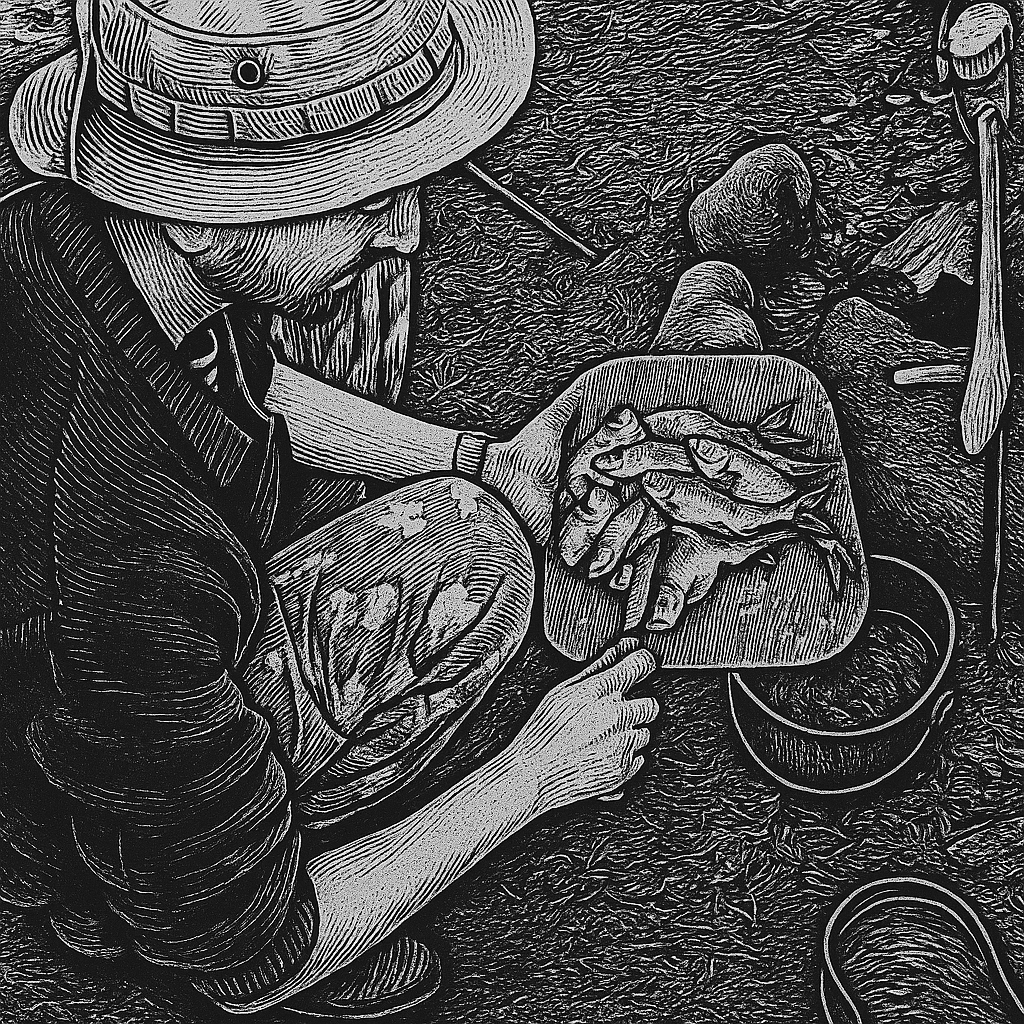
\includegraphics[width=1.0\textwidth]{8_5_new}
%	\caption{\small\textit{...А что там с супом?...}}
%	\end{figure}
%%\end{wrapfigure}
\diagdash Не с супом, а с ухой!\mdash Адмирал прикинул, что рыба целиком в котелок не влезет, взял байдарочное сиденье и~стал разрезать на нём чищенные рыбные тушки пополам.\mdash Руслан, подсоби! Давай сюда котелок, открывай.

Тот снял с костра котелок, а Адмирал присел и~стал аккуратненько ссыпать рыбу с байдарочного сиденья в~кипящую воду, где уже плавала полуготовая картошка и~зажарка, а потом засыпал кус\sdash куса для наваристости.

\diagdash Так, ну всё! Уха скоро подойдёт! А то уже восемь вечера, кушать охота! Тащ Замполит! Где знамя полка, ёпрст?! Разброд и шатание! 

%\newpage
%%\begin{wrapfigure}[12]{r}{0.5\textwidth}
%\begin{figure}[h]
%	\centering
%	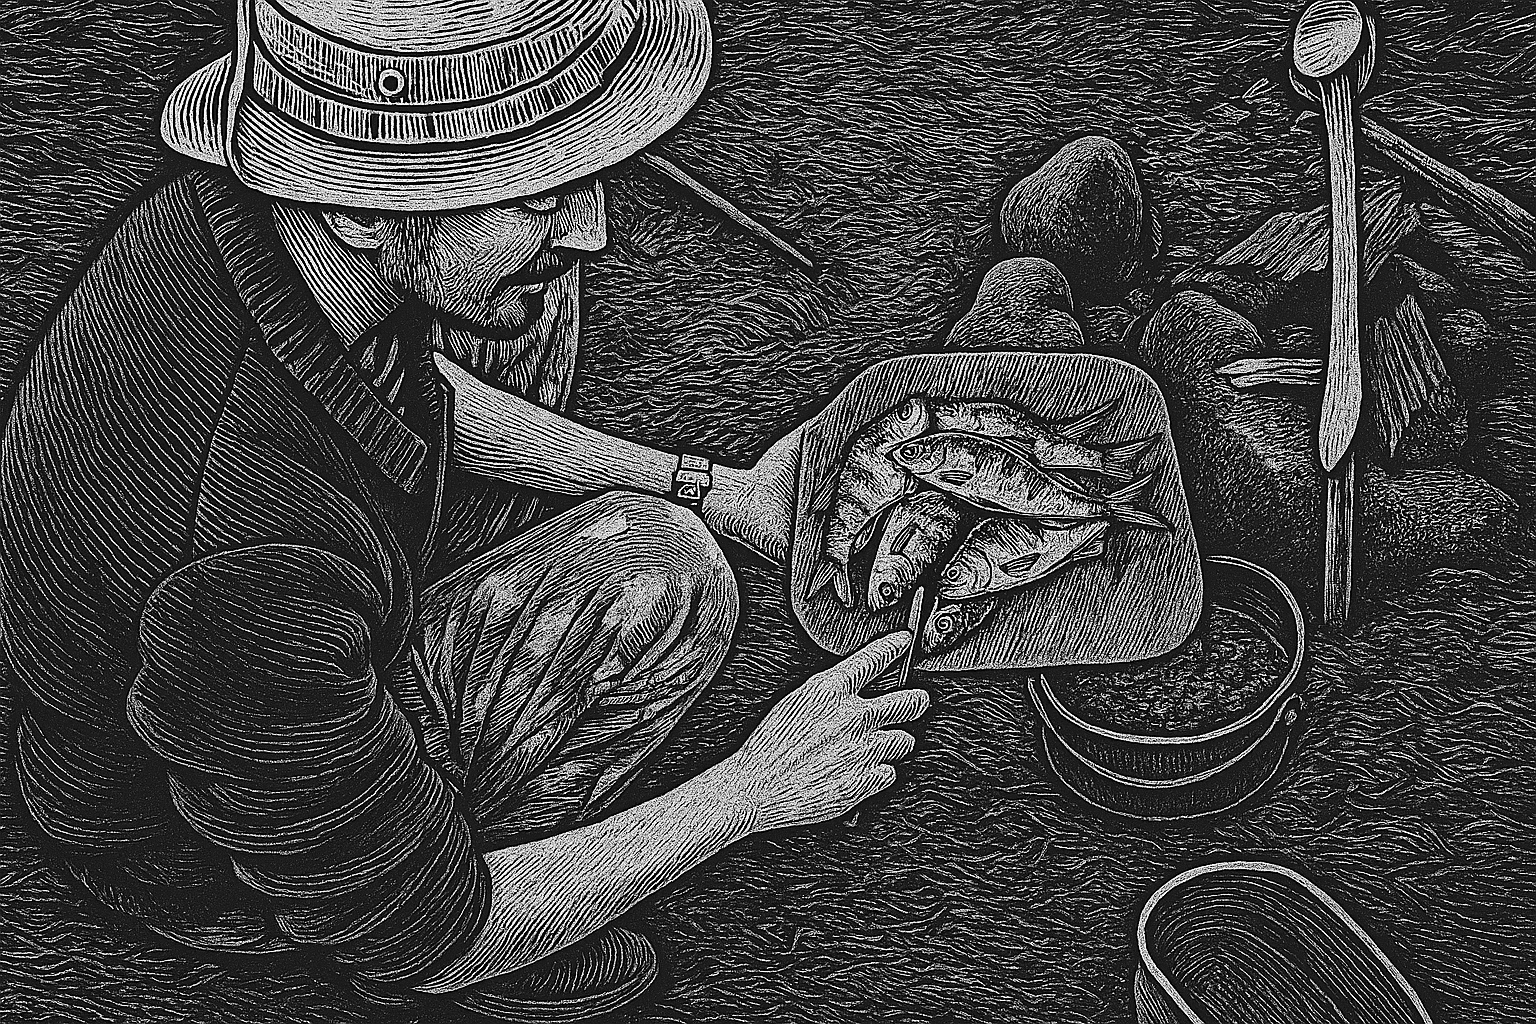
\includegraphics[width=1.0\textwidth]{8_5_new2}
%	\caption{\small\textit{...А что там с супом?...}}
%\end{figure}
%%\end{wrapfigure}

\diagdash Так вон же!\mdash на оттяжке тента, который давно растянули над столом и скамейками, красовалось знамя.

\diagdash Отлично! Щас дожариваем грибы и можно трапезничать!\mdash резюмировал Адмирал.

\diagdash А что это значит?\mdash мигом нарисовался Замполит.

\diagdash Значит разливай, ёпрст!

\diagdash Точно!

\newpage
%\begin{wrapfigure}[12]{r}{0.5\textwidth}
\begin{figure}[h]
	\centering
	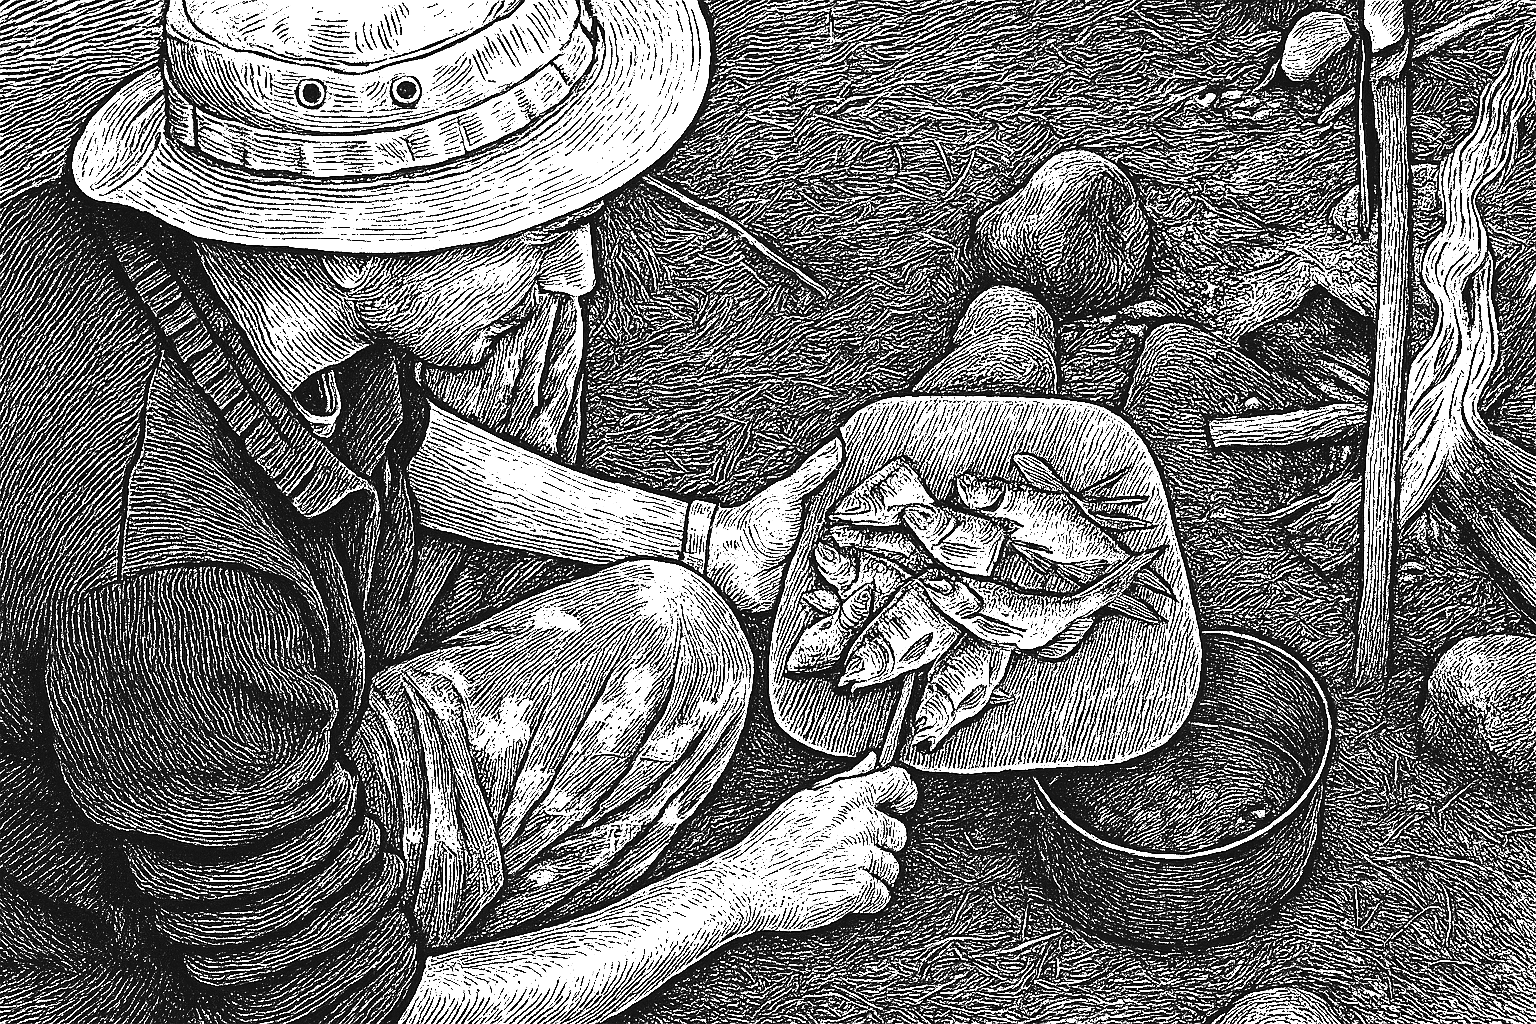
\includegraphics[width=1.0\textwidth]{20_1_fish}
	\caption{\small\textit{...А что там с супом?...}}
\end{figure}
%\end{wrapfigure}

Вокруг медленно спускалась ночь, хотя было довольно светло. Адмирал решил крестить уху, когда та сварилась\mdash присел у котелка, выбрал из костра горящее полено поухватистей с~угольком и, открыв флягу с водкой, многозначительно сказал:

\diagdash Ну!!!

\diagdash Шурик, ты ж это, как его, Иггдрасиль, Тор, {\'{O}}дин и~прочие?\mdash встрял Серёга.

\diagdash Пофиг, не мешай священнодейству!

Адмирал, взяв в правую руку дымящееся горящее полено, а в левую флягу, приступил. Он перекрестил уху и~размешал её дымящимся и шипящим поленом, одновременно подливая из~фляги.

\diagdash Всё, всё-ё-ё!\mdash Паша остановил процесс.\mdash Хар{\'о}ш!

\diagdash Нормально! Покрестили!\mdash Адмирал вытащил полено из~котелка.

\diagdash {\large УРА, УРА, УРА\sdash А\sdash А!!!}\mdash грянуло над озером.

\diagdash Давайте кушать! Дай половник, встаю на раздачу! Миски сюда!\mdash Замполит сел к костру и зазвенел половником по крышке котелка.

\diagdash Шу-у-урик, позволь заметить, это было как\sdash то не~по\sdash древнескандинавски!\mdash вставил Серёга.

\diagdash Да будет вам известно, достопочтенный Сергей, крест\mdash древний символ, и его христиане тоже, собственно, заимствовали в свой культ, как и многое другое, из~других религий и дохристианских верований, которые они впоследствии обозвали язычеством для очернения. Крест~использовали египтяне, ассирийцы, кельты, индусы и~вообще все кому не лень\mdash так что мне абсолютно~пофиг! 

Шурик окончил свою мини\sdash лекцию и команда стала разгульно трапезничать\mdash уха вышла навариста, даже слишком\mdash у Адмирала, видимо, дрогнула рука и он сыпанул в неё больше кус\sdash куса, чем следовало бы, но ребята всё равно умяли свои порции с~аппетитом, а~потом своей участи не избежала и~картошечка с~луком и~грибами. Веселье лилось рекой, апельсин, сало и~компотик уходили на~ура. Вдалеке над Мярандуксой взошла, почему\sdash то оранжевого цвета, Луна. Ночь окончательно накрыла своим крылом чертоги Мидгарда, ветер стих, темнота была как бы прозрачной и безмятежной.

%\newpage
Из колонки лился Цой, без которого, вне всяких сомнений, не обходились ни одни их посиделки, потому что это были песни их детства:

\vspace{0.1cm}
\noindent\textit{%
	\hspace*{2.0cm}Группа крови\mdash на рукаве,\\	
	\hspace*{2.0cm}Мой порядковый номер\mdash на рукаве,\\	
	\hspace*{2.0cm}Пожелай мне удачи в бою, пожелай мне\\
	\hspace*{2.0cm}Не остаться в этой траве$\ldots$
}
\vspace{0.1cm}

\diagdash Так, а ну-ка! Пожелай мне конфэт! В каком мешке конфэты?\mdash Паша виляющей походкой побрёл копаться в~продуктовых гермах.

\diagdash В зелёной вроде, там же подписано.\mdash ответил Адмирал.

\diagdash Да не видно уже, темно!

\diagdash Те посветить?\mdash Адмирал, шатаясь, поднялся от~стола.\mdash Во,~чё~играет! Дава\sdash а\sdash а\sdash ай! Зажигай, народ!\mdash из~колонки неслось:

\vspace{0.1cm}
\noindent\textit{%
	\hspace*{2.5cm}С причала рыбачил апостол Андрей,\\	
	\hspace*{2.5cm}А Спаситель ходил по воде.\\
	\hspace*{2.5cm}И Андрей доставал из воды пескарей$\ldots$	
}
\vspace{0.1cm}

\diagdash П-пацаны, по в-воде ход-дить не будем!\mdash Замполит наворачивал закусь.

\diagdash Карма наша не настолько чиста, не выдержит тебя гладь водная! Чи\sdash и\sdash исть карму!\mdash Адмирал, нацепивший свою любимую раста\sdash шапку, которую ему собственноручно связала жена, уже словил дзен, сидя на~скамейке, поджав ноги под себя на манер позы лотоса.\mdash Ом\sdash м\sdash м!

\diagdash А пескарей сегодня Паша и так натягал вон на целый котелок! Уха навариста вышла!

\diagdash Не пескарей, а к-краснопёрок и плотвы!\mdash поправил Паша, роясь в герме. Конфеты сползли на~самое дно и никак не хотели доставаться. Наконец, найдя полиэтиленовый мешочек со~сладостями, они c~Адмиралом вернулись, колбасясь под музон, ко столу:

\diagdash Сударь! Плесните?

\diagdash Ессесно!

Вторая стоянка вышла у них на отлично\mdash искупались, рыбы наловили, ухи наварили, картохи с грибами нажарили, у костра попели\sdash поорали. Плейлист закончился, колонку они выключили. Ближе к полуночи Замполит смазал картину тем, что дошёл до точки:

\diagdash Тэк\sdash с, Шурик, я чёта всё!

\diagdash Аллё, ты чё? Пойдём подышим ночным воздухом!\mdash Шурик потащил Кирю подальше от костра:

%\newpage
\vspace{0.1cm}
\noindent\textit{%
	\hspace*{2.0cm}Вы вертикальной плоскости держитесь,\\	
	\hspace*{2.0cm}Определите, что это за жидкость?\\	
	\hspace*{2.0cm}Конечно спирт, вы, видно, парень тёртый,\\	
	\hspace*{2.0cm}И ставлю я вам твёрдую пятерку$\ldots$	
}
\vspace{0.1cm}

\diagdash Вы ток там с берега не ломанитесь!\mdash донеслось до~них.

%\renewcommand*{\thefootnote}{\arabic{footnote}}
\renewcommand*{\thefootnote}{\fnsymbol{footnote}}
\setcounter{footnote}{0}
Спустя полчаса Кирю попустило, Шурик потащил его обратно к костру. Выглядели они комично\mdash Киря в~белой футболке, а Шурик в тельняшке навыпуск, оба с налобными фонариками, ну вылитая Кин\sdash дза\sdash дза\footnote{Советская двухсерийная трагикомедия в жанре фантастической антиутопии, снятая режиссёром Георгием Данелией на <<Мосфильме>> в~1986 году.}, петляющей походкой шатались они по лесу, стараясь не упасть. Пашка уже пошёл спать, как и Руслан. Серёга допил компот, прибрался на~столе и уже пошёл к своей палатке. И тут два абстрактных тела вернулись к~столику:

\diagdash Так! Пей компотик!\mdash насел Адмирал на Замполита, зачерпнув ему в кружку из котелка.

\diagdash Не хочу!

\diagdash Пей компотик!

\diagdash Не хочу!

\diagdash Кирь, я тя поколочу щас! Пей компотик!

\diagdash Шурик, отстань, не хочу!

\diagdash Пей компотик, полегчает!

\diagdash Пацаны, чё у вас там?\mdash Серёга вернулся к столу.\mdash Ё\sdash ё\sdash ё, Киря$\ldots$

\diagdash Всё норм! У нас тут это, алкоголики, тунеядцы, хулиганы$\ldots$ \mdash Адмирал придерживал Замполита чтоб тот не~упал.

\diagdash А-а-а, ну тогда всё в порядке. Давайте, чао, парни, я~спать!\mdash и Серёга ушёл.

%\newpage
%\begin{wrapfigure}[12]{r}{0.5\textwidth}
%\begin{figure}[h]
%	\centering
%	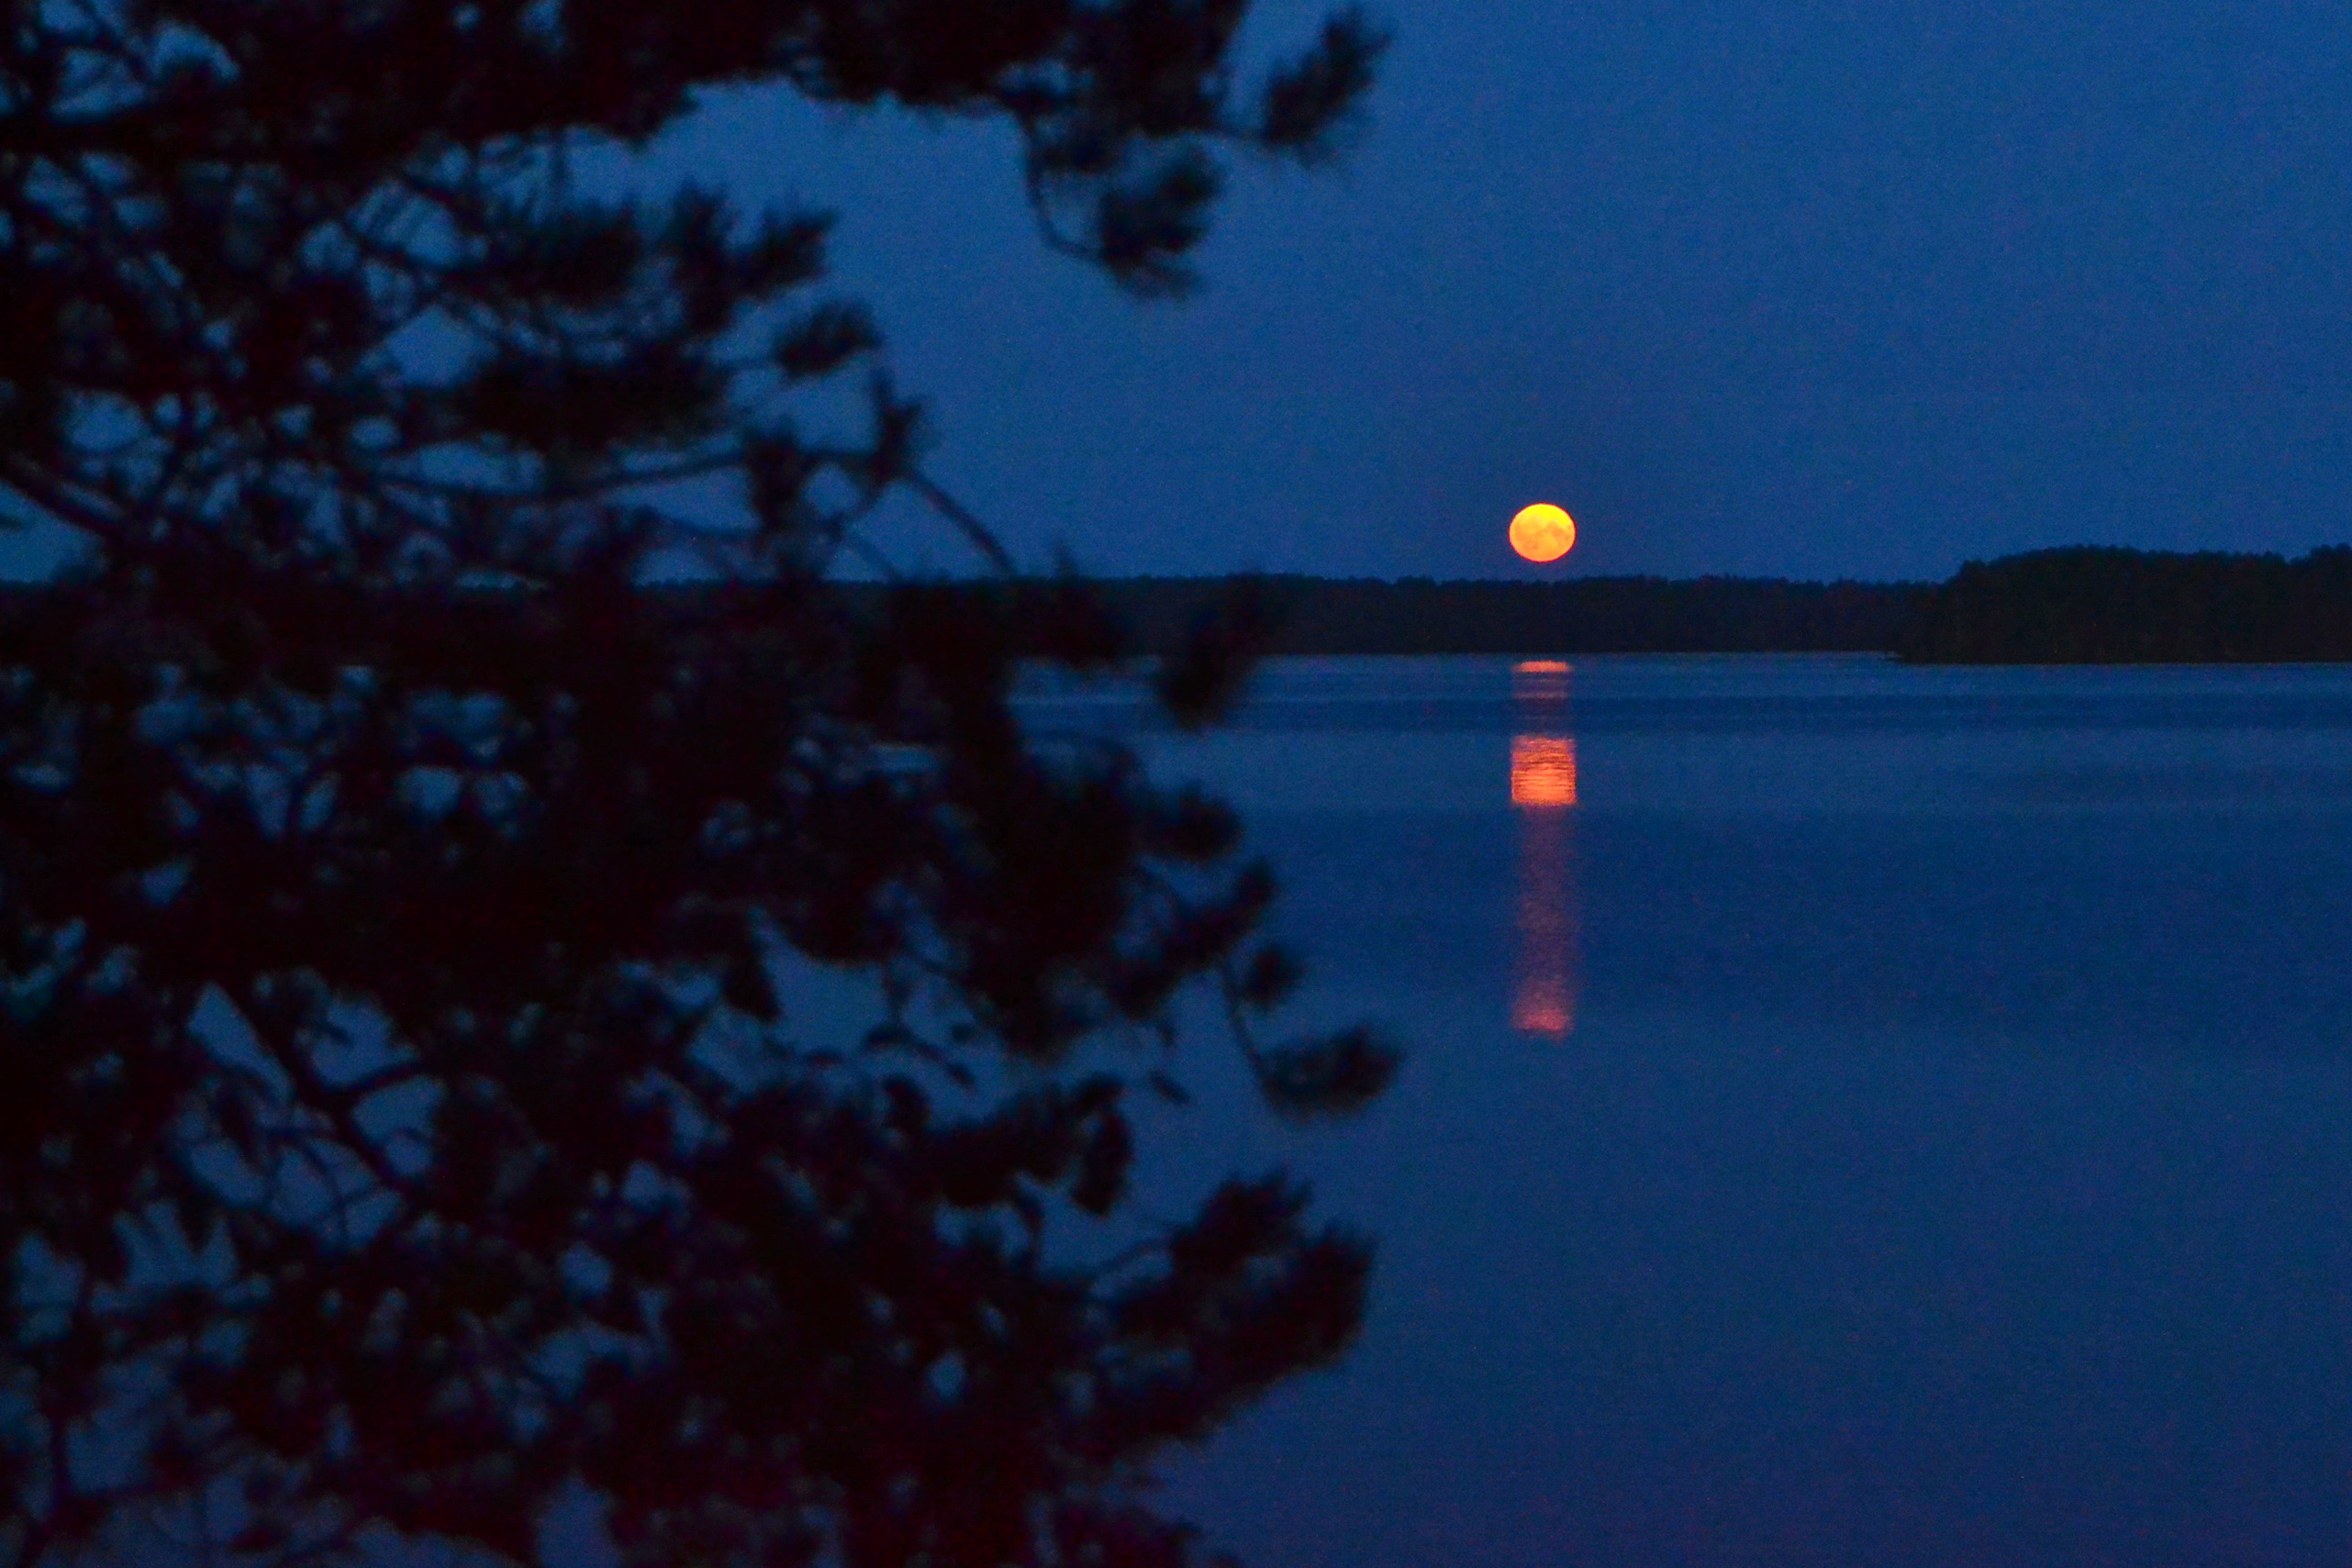
\includegraphics[width=1.0\textwidth]{8_6}
%	\caption{\small\textit{...Луна, взошедшая над лесом, отражалась в Мярандуксе...}}
%\end{figure}
%\end{wrapfigure}

Остались только Адмирал с Замполитом у костра: 

\setlength{\belowcaptionskip}{-10pt}
\begin{figure}[h]
	\centering
	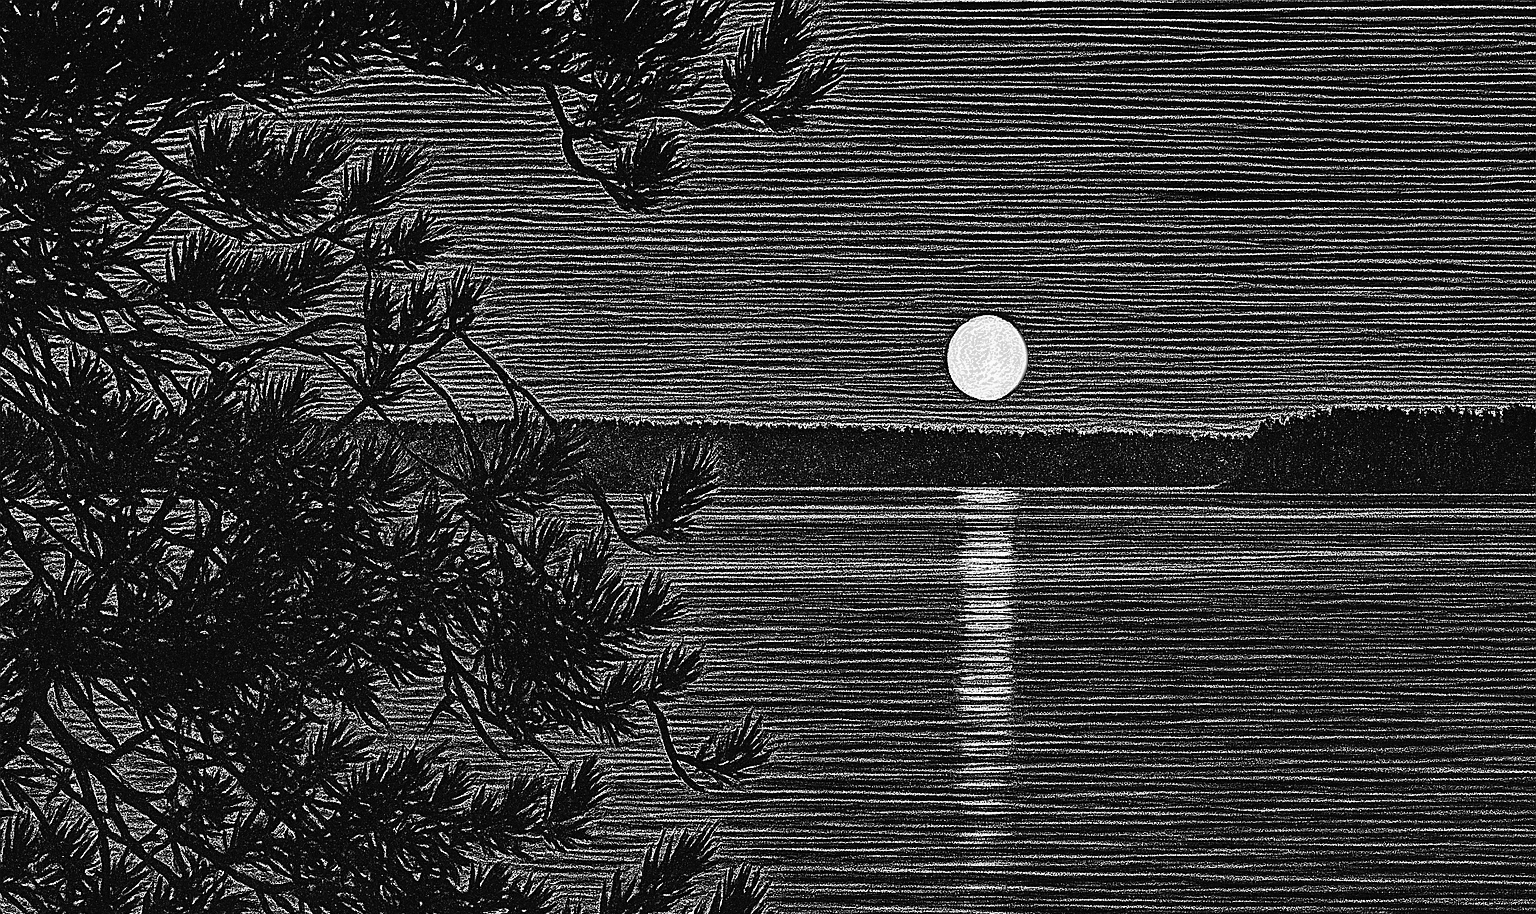
\includegraphics[width=1.0\textwidth]{21_moon.png}
	\caption{\small\textit{...Луна, взошедшая над лесом, отражалась в Мярандуксе...}}
\end{figure}

\diagdash Пей компотик!\mdash наседал Адмирал.

\diagdash Не хочу!

\diagdash Пей компотик!

\diagdash Не хочу!

\diagdash ТАК!!!

\diagdash Ладно$\ldots$\mdash сдался Замполит.

%\begin{figure}[h]
%	\centering
%	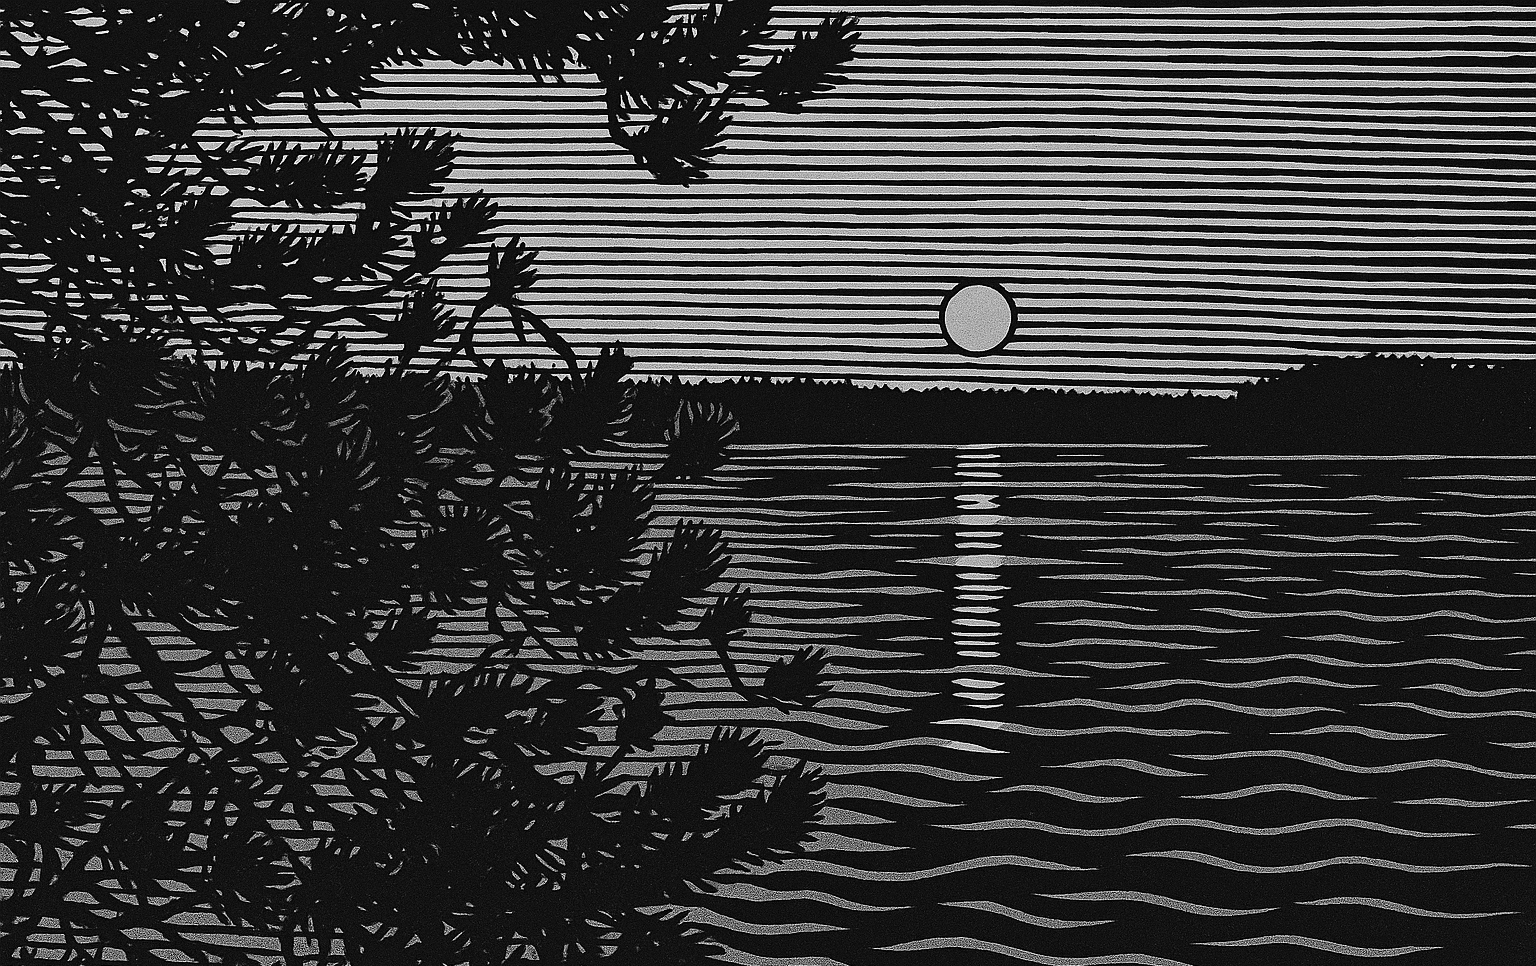
\includegraphics[width=1.0\textwidth]{8_7_new1}
%	\caption{\small\textit{...Луна, взошедшая над лесом, отражалась в Мярандуксе...}}
%\end{figure}

%\newpage
Ночь наконец\sdash то стала по\sdash настоящему тёмной. Без~фонарика\mdash ни~зги не~видно. Они сидели к плечу плечо на~лавочке спиной к~столу, обратив свой взор на~ночную озёрную гладь, простиравшуюся перед ними. Луна, взошедшая над лесом, отражалась в Мярандуксе, создавая едва дрожащую световую дорожку. Воздух~наполнился ночной влагой и ароматами воды, хвои\mdash ничто не могло заглушить этот божественный запах природы. Вокруг была настолько вакуумная тишина, что временами было непонятно, остались ли в принципе какие\sdash то звуки, или это обогащённая спиртом кровь бежит по~сосудам в ушах.

%тишь да~гладь, красотища. 

%\begin{figure}[h]
%	\centering
%	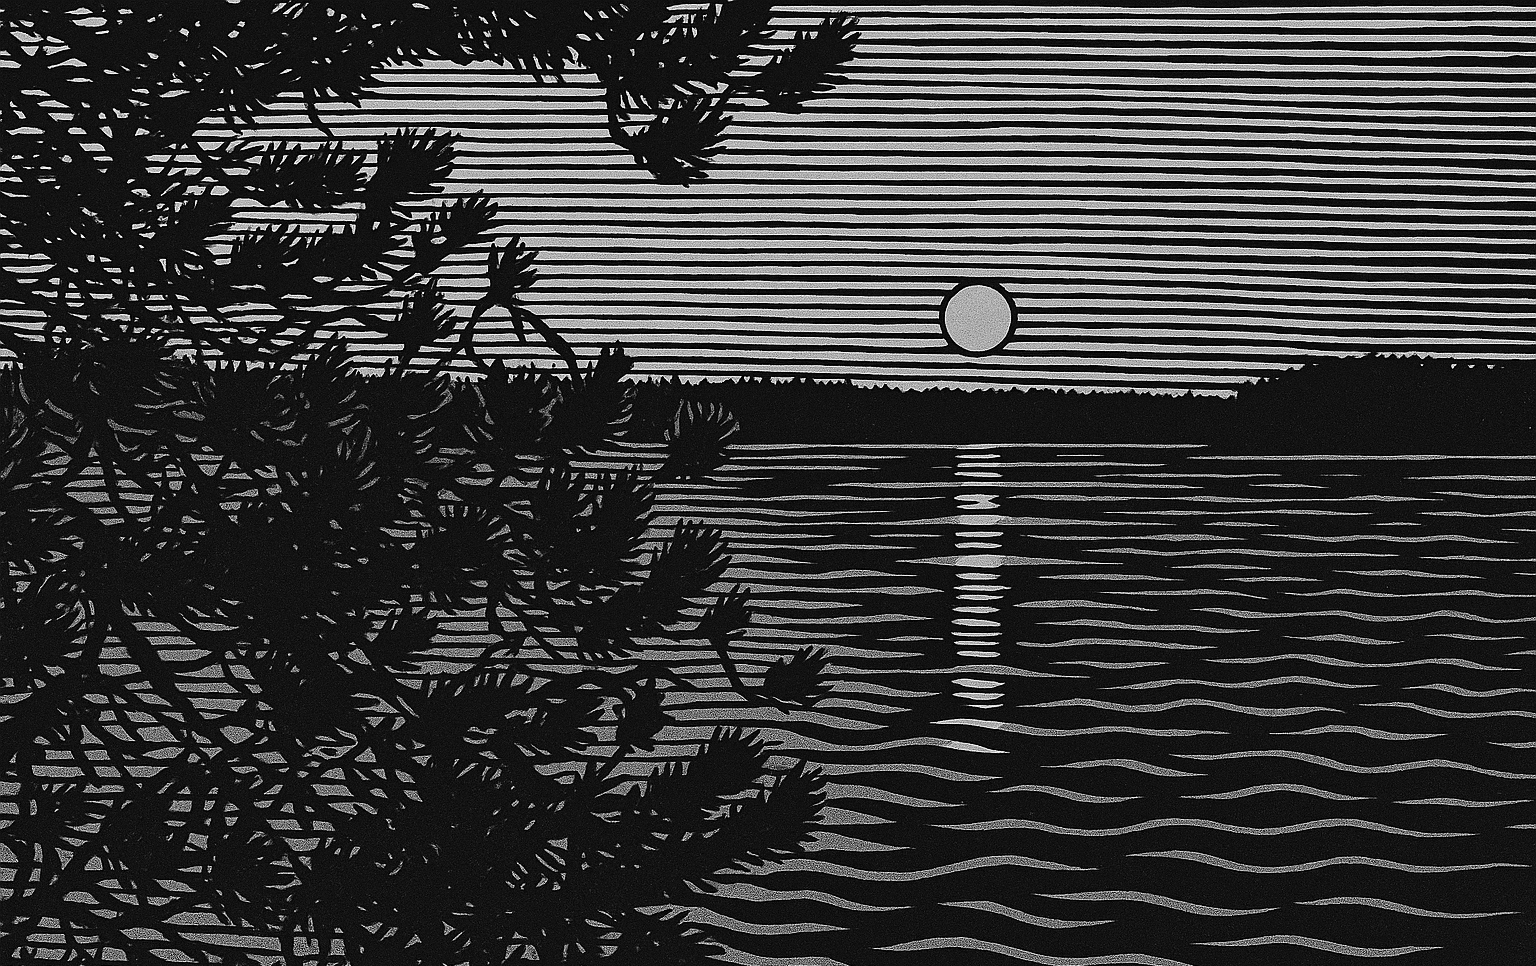
\includegraphics[width=1.0\textwidth]{8_7_new1}
%	\caption{\small\textit{...Луна, взошедшая над лесом, отражалась в Мярандуксе...}}
%\end{figure}

Понемногу Кире стало получше, а с небес начал накрапывать лёгкий дождичек. Костёр почти догорел, угли подёрнулись пеплом. Шурик сидел на~лавочке, смотрел на~озеро, задумчиво смолил и~попивал компотик$\ldots$



\begin{center}
	\psvectorian[scale=0.4]{88} % Красивый вензелёк :)
\end{center}
